\chapter[IDEA DR calorimeter simulation]{IDEA dual-readout calorimeter simulation and SiPM signal digitisation}
%As already said, the conceptual experiment described in Section \ref{sec:Idea_project} is an ongoing project and it has to be supported by simulation. With this goal, a dual-readout calorimeter full simulation has been developed allowing to generate data and monitor the whole process from the collision at the interaction point to the digitized signal produced by SiPMs.\\
As already said, a full simulation of the dual-readout calorimeter performance has been implemented. It has been done, in particular, in the context of the R\%D work for the preparation of the Conceptual Design Reports (CDRs) and, next, of the Technical Design Reports (TDRs) for both FCC-ee and CEPC. The simulation includes the showering of particles in the detector and the generation and transport of photons till the readout sensors. Finally, the photon time of arrival is used to trigger the simulation of the sensor response which has been extensively studied for this thesis.\\

The chapter presents a description of the simulation chain. The Section \ref{sec:Sim_struc} describes in details the simulation dividing it in two main Monte Carlo processes:
\begin{itemize}
	\item the calorimeter simulation, coded in C++ using the GEANT4 toolkit;
	\item the SiPM response digitisation, coded in a dedicated Python application.
\end{itemize}

Important aspects of the SiPM response, such as the temporal behaviour, the SiPM non-linear response and the energy resolution will be described in Section \ref{sec:Sim_perf}.\\

%The calorimeter structure opens various possibility for the identification of isolated primary particles using neural network structures. This topic will be deeper treated in the next chapter.\\
The SiPM readout, in which each fibre is coupled to a dedicated SiPM, gives the possibility to sample showers with a unprecedented 2D granularity.
In this context the usage of deep neural networks for particle identification studies has been pioneered and will be discussed in the next chapter.


\section{Simulation structure} \label{sec:Sim_struc}

\subsection{Calorimeter simulation} \label{subsec:Sim_cal}
The simulated calorimeter structure follows the conceptual design shown in Section \ref{sec:Idea_project}. It has a cylindrical symmetry characterised by a barrel and two end-cap regions. This $4\pi$ structure is obtained through $36$ discrete rotations, around the $z$ axis, of a  simpler unit, called a slice. The dimensions of each slice are shown in Figure \ref{fig:cal_slices}. The inner diameter and  the inner length are both $5$ m, and the overall outer diameter and length are $9$ m.\\
Each half slice is composed by 75, $2$ m long, towers ($40$ in the barrel and $35$ in the endcap region) and a total of $5400$ towers compose the whole calorimeter.
To cover a solid angle very close to $4\pi$, each tower has a different trapezoidal inner face with dimensions that can vary from $\sim 5$ cm to $\sim 8$ cm. The coverage in $\theta$ is down to $\sim 0.1$ rad from the beam line.\\

%\begin{figure}
%	\centering
%	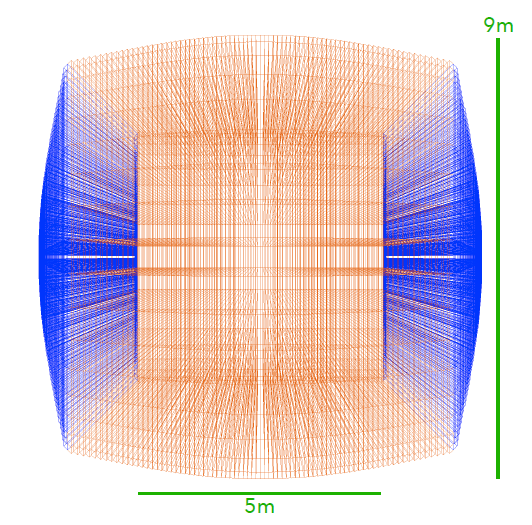
\includegraphics[width=0.6\textwidth]{IMG/DRCGeometry3}
%	\caption{Calorimeter geometry.}
%	\label{fig:cal_geometry}
%\end{figure}
\begin{figure}
	\centering
	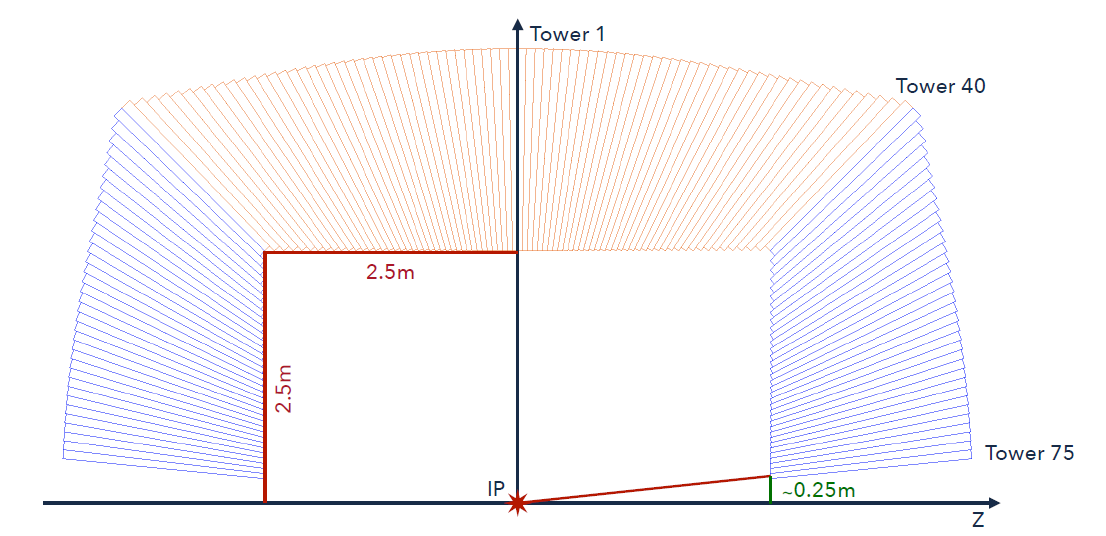
\includegraphics[width=0.8\textwidth]{IMG/DRCGeometry1}
	\caption{A calorimeter slice.}
	\label{fig:cal_slices}
\end{figure}

At present, towers are copper-based with fibres inserted in a chessboard-like geometry. Longitudinally running holes host optical fibres as sensitive elements. The need of a projective geometry makes the detector dimensions increasing with the distance from the IP. New holes (with new fibres) open up at different depths inside the calorimeter, whenever possible, to keep the sampling fraction constant.\\
As the dual-readout technique needs independent scintillating ($S$) and Cherenkov ($C$) signals, two types of fibres are used (Fig. \ref{fig:CS_fibres}). Their characteristics are shown in Tab. \ref{tab:fibres}.\\
The fibre refractive indices determine the light collection capability, as dictated by Snell's law. The signal from the scintillating fibres is parametrised by the deposited energy while the Cherenkov photons are produced accordingly to the Cherenkov emission process.\\

\begin{table}
	\centering
	\setlength{\tabcolsep}{12pt}
	\begin{tabular}{lp{0.6\textwidth}}
		\toprule
		\multicolumn{2}{c}{\textbf{Kuraray SCSF-78 ($S$)}}	\\
		\midrule
		Core:				& $r = 0.485$ mm, Polystyrene ($C_5H_5$), $\rho=1.95$ g$/$cm$^3$, $n = 1.59$	\\
		Cladding: 			& Thickness $=2\%$ of $r$, PMMA ($C_5H_8o_2$), $\rho=1.19$ g$/$cm$^3$, $n=1.49$	\\
		Main properties:	& Emission constant $= 2.8$ ns, LY $= 10^4$ photons$/$MeV, $\lambda_{att} = 4$ m	\\
		\midrule
		\multicolumn{2}{c}{\textbf{Mitsubishi SK-40 ($C$)}}	\\
		\midrule
		Core:				& $r = 0.485$ mm, PMMA ($C_5H_8o_2$), $\rho=1.19$ g$/$cm$^3$, $n = 1.49$	\\
		Cladding: 			& Thickness $=2\%$ of $r$, Fluorinated Polymer ($C_2F_2$), $\rho=1.43$ g$/$cm$^3$, $n=1.42$	\\
		Main properties:	& $\lambda_{att} = 8.9$	m\\
		\bottomrule
	\end{tabular}
	\caption{Technical characteristics of the two type of fibres used.}
	\label{tab:fibres}
\end{table}

\begin{figure}
	\centering
	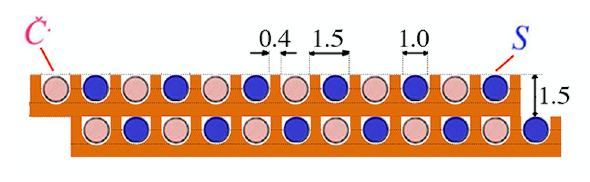
\includegraphics[width=0.8\textwidth]{IMG/DRCGeometry2}
	\caption{Chess-like configuration to dispose fibres in the copper structure.}
	\label{fig:CS_fibres}
\end{figure}

For each event, the simulation produces as output the following information per each activated fibre: 
\begin{itemize}
	\item Event ID;
	\item Fibre Type ($C$ or $S$);
	\item Fibre ID (a unique number per fibre);
	\item the $(x,y,z)$ position of the fibre tip closer to the IP;
	\item the number of photons reaching the SiPM;
	\item the list of photon times of arrival to the SiPM.
\end{itemize}

The computation of the light propagation inside fibres is extremely time consuming, so that it has to be fine tuned in order to optimise the full process. In particular, the propagation of $C$ photons is tracked until the single photon reach the core-cladding boundary. If the emission angle is inside the range of the fibre numerical aperture, the photon is added to the final number of photons. Following a Poissonian probability smearing of being detected, each photon is converted to a photoelectron (p.e.).
The time of arrival on the sensor for each photon is estimated as:
\begin{equation}
t_C = t_0 + R \frac{n_C}{c\cdot \cos(\vartheta)}
\end{equation}
where $n_C = 1.49$ is the fibre refractive index, $c$ the speed of light, $R$ the distance from the further end of the fibre and $t_0$ the time at which the photon reach the core-cladding boundary.\\

For the $S$ fibres, instead, the photons are produced by weighting the light yield of the fibres with the actual energy deposited by the interacting particle. The number of photons is smeared with a Poissonian law for the photoelectron conversion and the time of arrival on the sensor is obtained as:
\begin{equation}
	t_S = t_0 + R\frac{n_S}{c\cdot \cos(\vartheta)} + t^*
\end{equation}
where $n_S = 1.59$ is the refractive index and $t^*$ a random time that accounts for the scintillator decay time, chosen from an exponential distribution with $2.8$ ns as mean value.
Considering the internal reflection, the photon path depends on the $\vartheta$ angle (i.e. the angle between the photon direction and the fibre axis). It is chosen randomly in the range $[\cos(\alpha),\cos(0)]$, where $\alpha = 20.4\degree$ is the fibre critical angle.\\
Eventually, the light produced is smeared by two Poissonian distribution, one for the scintillation signal and the other for the Cherenkov one. This procedure correctly reproduces the statistical fluctuations in the scintillation and Cherenkov light production and allows to reproduce within the simulations the desired light yields (p.e./GeV).
%To make the full simulation lighter, this process also includes the attenuation due to the PDE of the simulated SiPMs.
The simulation is tuned to produce $\sim 400$ Spe$/$GeV and $\sim 100$ Cpe$/$GeV at the electromagnetic scale. (i.e. for em showers).

\subsection{SiPM response digitization} \label{subsec:Sim_SiPM}
The output of the G4 simulation is used as input of the second part of the simulation: \textit{pySiPM}, a python-based Monte Carlo simulation able to reproduce the SiPM transfer function and extract features from the waveforms recorded with a digitiser \cite{digitizer}.\\

The importance of this software goes beyond our context, but perfectly fits our needs. In particular each fibre from the calorimeter simulation is considered as coupled to a single SiPM, whose signal is simulated through \textit{pySiPM} in each event.

The simulation allows to set most of the SiPM parameters:
\begin{itemize}
	\item \textbf{Geometrical parameters}: the sensor dimensions and the pixel pitch.
	\item \textbf{Sensor parameters}: Photon Detection Efficiency, Dark Count Rate, After-Pulse probability, Optical Cross-Talk probability.
	\item \textbf{Signal parameters}: rise time constant, decay time constant.
	\item \textbf{Waveform parameters}: sampling frequency, integration time window, integration starting time.
\end{itemize}

For each event and fibre, random parameters determine the photon position inside the sensor. %Meanwhile the sensor PDE is tuned to have consistent mean values of $\sim 400$ Spe$/$GeV and $\sim 100$ Cpe$/$GeV respectively for $S$ and $C$ light yield.
Meanwhile the sensor PDE is set at $100\%$ since the actual PDE is accounted within the poissonian smearing applied at the calorimeter simulation level.
%A control stops the count of impinging photons on the same cell to a maximum of one, then each element of noise is generated with the set probability.\\
When a photon impinges on a cell, a control is activated preventing the production of a new signal from the same cell. The control is removed after the recovery time of the cell set at $10\cdot \tau_{fall}$.\\

The photon times of arrival to the SiPM surface are synchronised to a common time trigger (in our case, the production of the particle at the interaction point). To be consistent with this time-zero (TZ) definition, the ToAs are passed to the digitiser software and used to start the avalanche discharge simulation at the exact time. In this way all the digitised waveforms are synchronised to the same TZ as defined by the GEANT4 trigger.\\

The generated pulse is a combination of two exponentials characterised by the rise time constant ($\tau_{rise}$) and the decay time constant ($\tau_{fall}$):
\begin{equation}
	f(t)= A \cdot \left( e^{-\frac{t + t_0}{\tau_{fall}}} - e^{-\frac{t + t_0}{\tau_{rise}}}\right),
	\label{form:resp_func}
\end{equation}
where $t_0$ is the photon time of arrival on the SiPM surface.\\
The output signal for any given SiPM is the sum of all the signals generated by the activated cells.\\

The information given as output of the SiPM simulation are:
\begin{itemize}
	\item \textbf{Data reported from GEANT4 simulation}: event ID, type of fibre, fibre ID, fibre position;
	\item \textbf{Computated quantities}: signal integral, peak height, time of arrival, time over threshold, time of peak;
	\item \textbf{Digitised waveform}.
\end{itemize}

It is also possible to select an analog threshold on the signal height to establish if information has to be recorded.
The threshold is defined as a scale factor of the maximum value of the waveform generated by a single photoelectron (neglecting the electrical noise). In the results shown later a 1.5pe-suppression has been applied using a threshold of $1.5$ of the signal height from a single photon. Such a filter is useful to neglect signals from DCR.\\

\section{Results from the full simulation chain} \label{sec:Sim_perf}

\subsection{Different configurations} \label{subsec:SiPM_conf}
The results shown in this chapter are obtained considering different SiPM parameter configurations.\\
They have been chosen in a common parameter space identified by checking the portfolio of SiPMs produced by Hamamatsu \cite{SiPM_lineup}. 
Two are the parameters that have been changed in our studies: 
\begin{itemize}
	\item the decay time constant of the signal, the selected values being $10$ ns and $50$ ns;
	\item the pixel size, the selected values being $10$ $\mu$m, $15$ $\mu$m and $25$ $\mu$m.
\end{itemize}

The other parameters have not been modified for this work. Their values are listed in the Table \ref{tab:SiPM_par}.\\

\begin{table}
	\centering
	\setlength{\tabcolsep}{18pt}
	\begin{tabular}{ll}
		\toprule
		\multicolumn{2}{c}{\textbf{Geometrical Parameter}}	\\
		SiPM area	& $1 \times 1$ mm$^2$	\\
		\midrule
		\multicolumn{2}{c}{\textbf{Sensor Parameters}}	\\
		DCR			& $200$ kHz	\\
		After-Pulse	& $3\% $	\\
		Cross-Talk	& $1\% $	\\
		\midrule
		\multicolumn{2}{c}{\textbf{Signal Parameter}}	\\
		Rise time	& $1$ ns	\\
		\midrule
		\multicolumn{2}{c}{\textbf{Waveform Parameters}}	\\
		Time window	& $500$ ns	\\
		Integration window	& $300$ ns	\\
		Sampling frequency	& $10$ GHz	\\
		\bottomrule
	\end{tabular}
	\caption{SiPM parameters kept constant in the simulation configuration file. For the values of the parameters that have been varied see the text.}
	\label{tab:SiPM_par}
\end{table}

An example of generated waveform, in response to $3$ simultaneous photoelectrons with a time of arrival of $20$ ns, is plotted in Figure \ref{fig:diff_wf}. The impact of the two different decay-time constants is evident.\\
Other waveform examples are shown in Figures \ref{fig:wf_dcr} and \ref{fig:wf_ap}, where signals generated by DCR and after-pulse noise, respectively, are included.\\

\begin{figure}
	\centering
	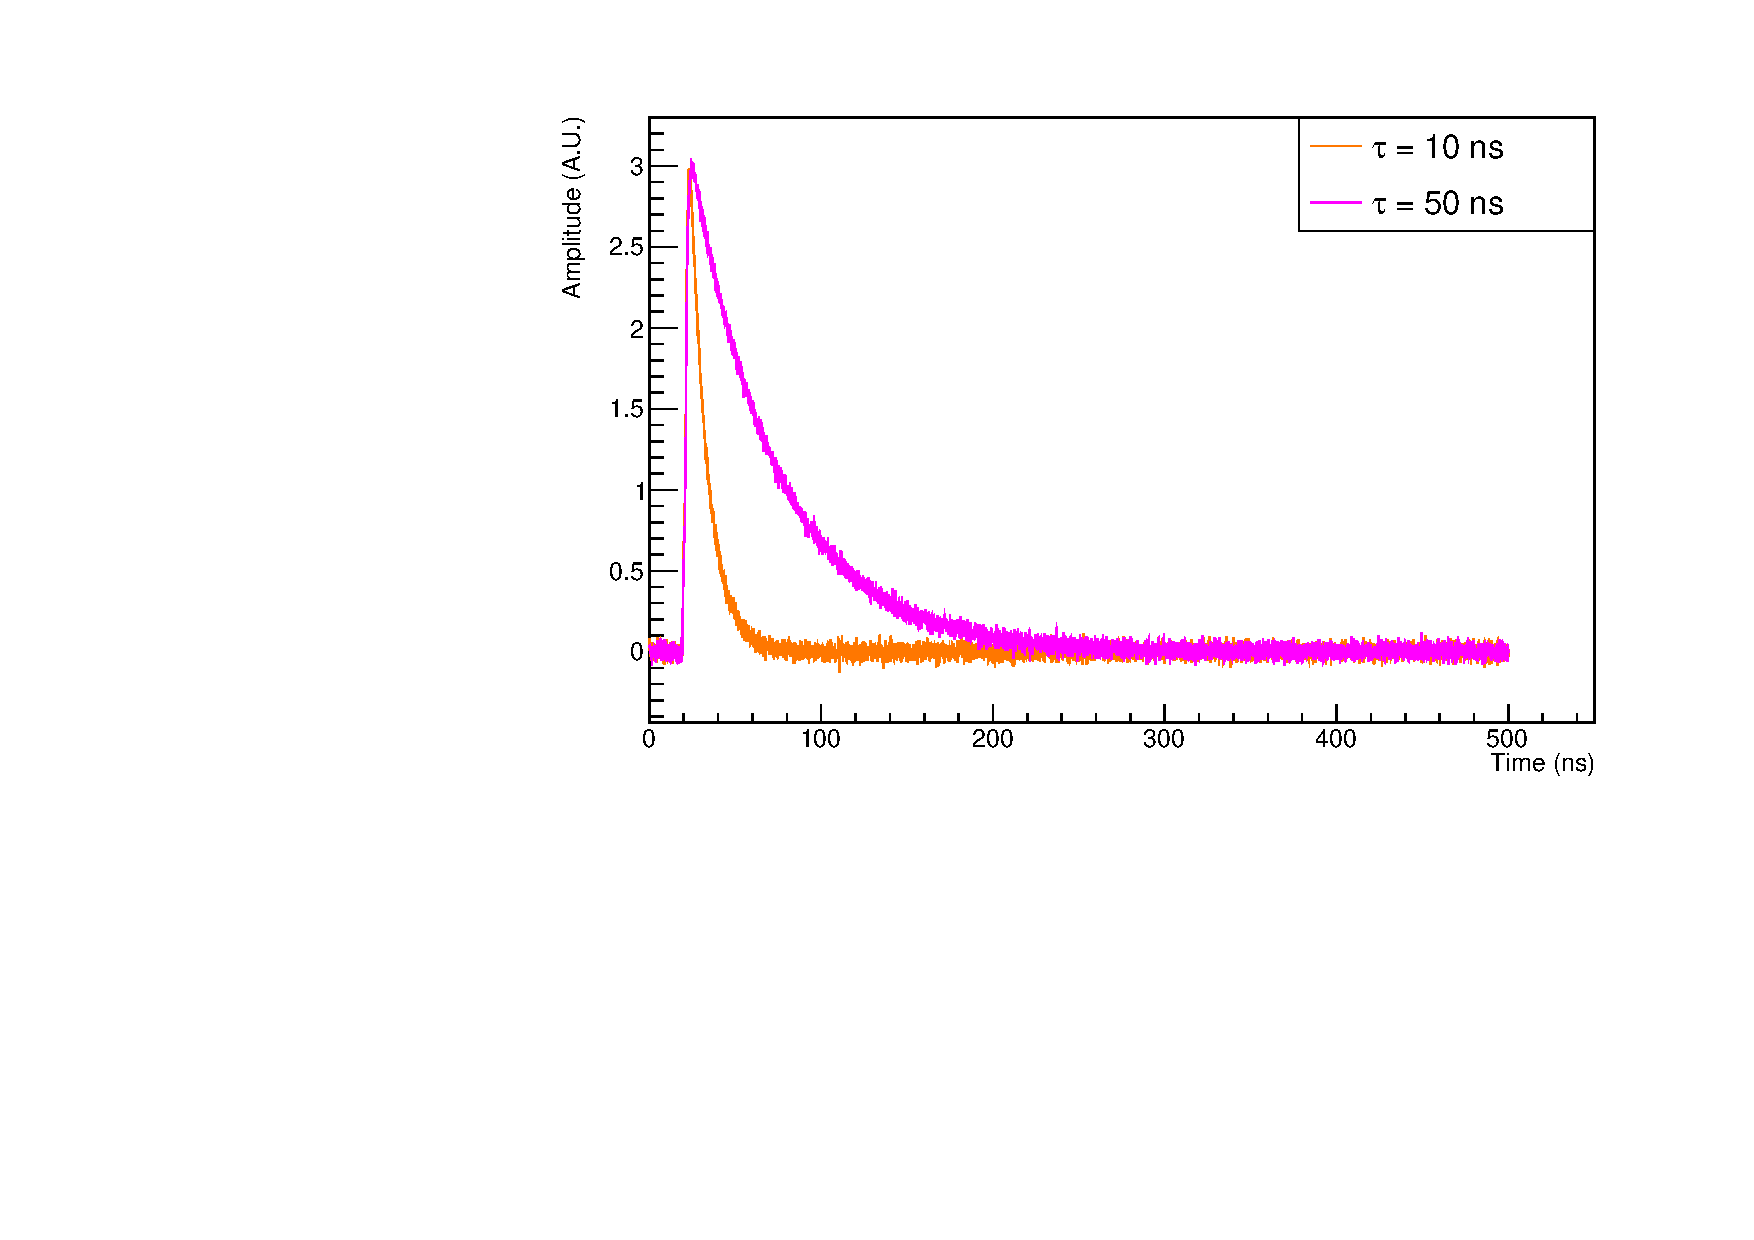
\includegraphics[width=0.8\textwidth]{IMG/Cap5/wf_different_conf}
	\caption{Single waveforms generated in response to $3$ simultaneous photoelectrons with time of arrival of $20$ ns while considering two identical conditions except for the decay-time constant.}
	\label{fig:diff_wf}
\end{figure}

\begin{figure}
	\centering
	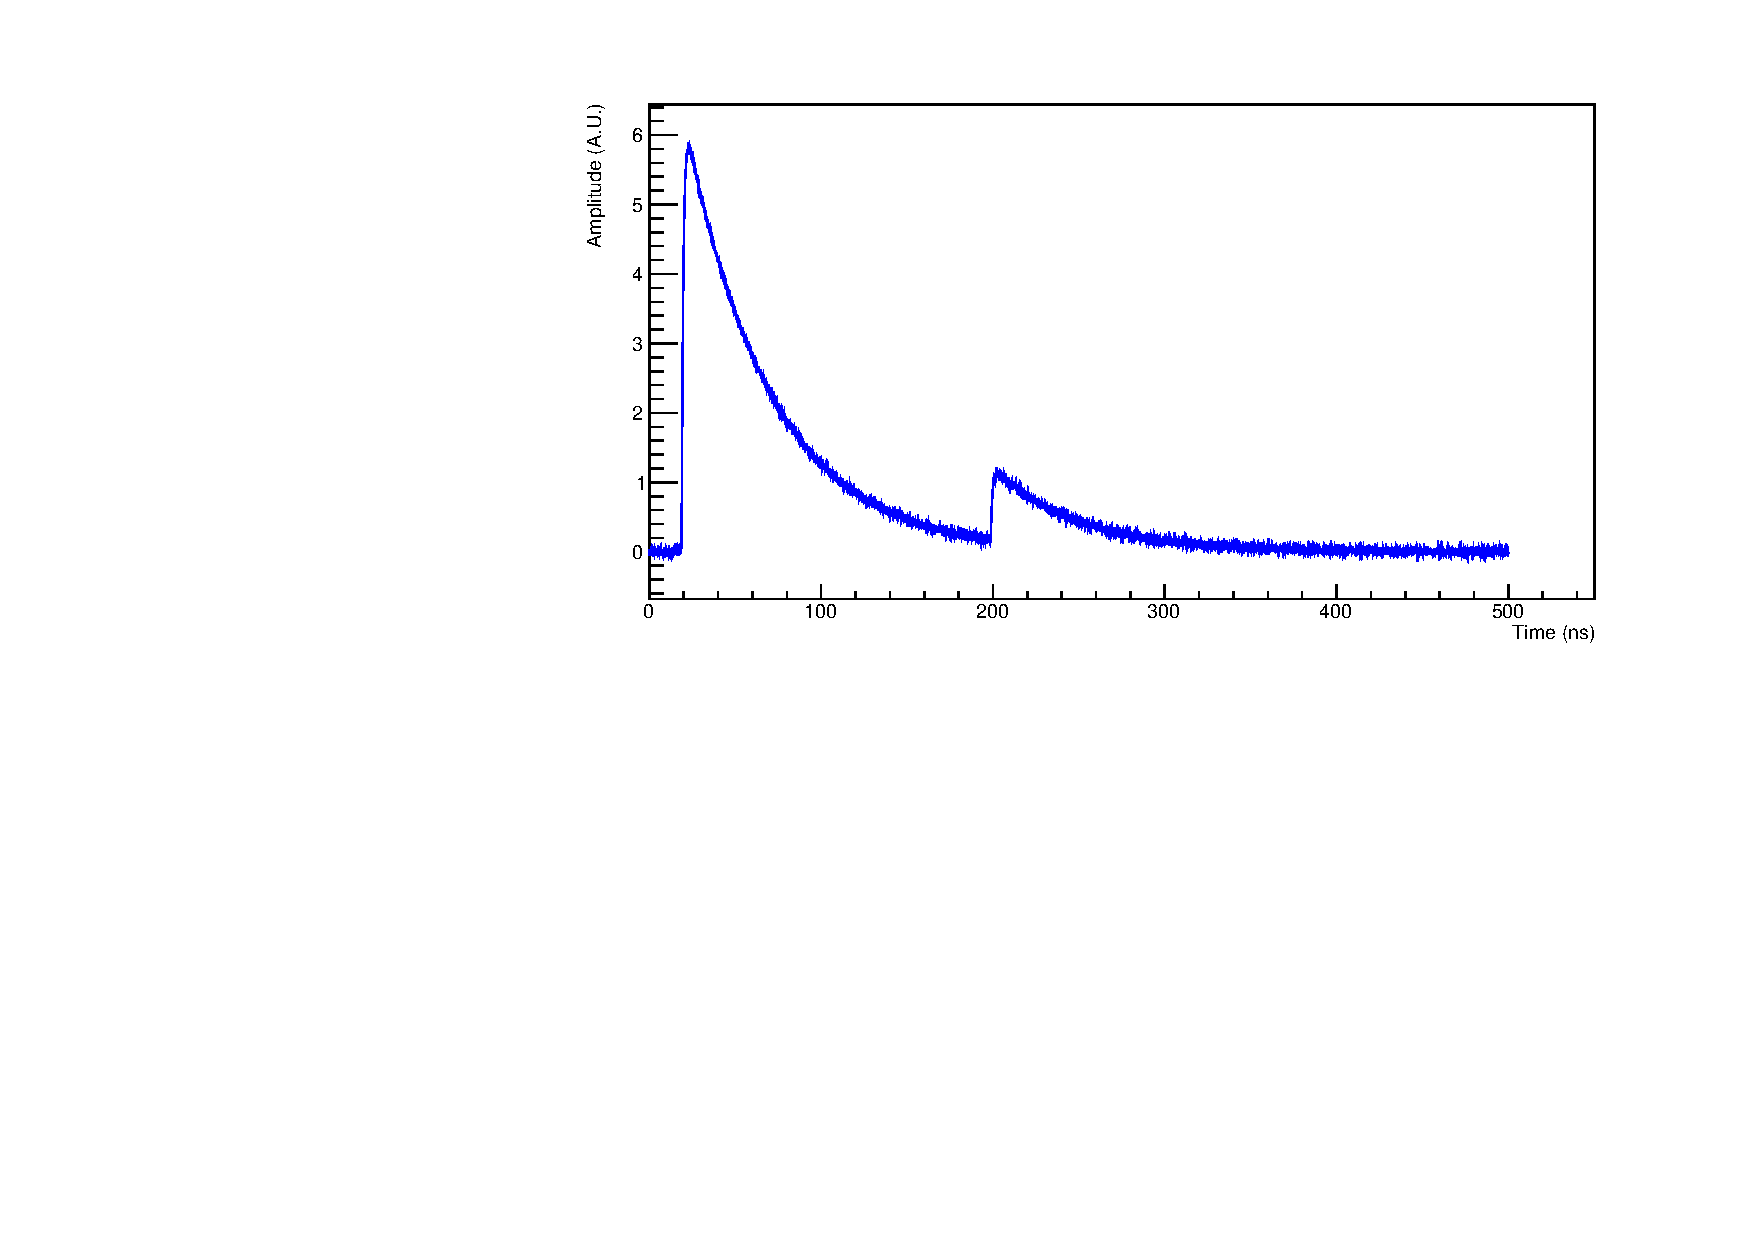
\includegraphics[width=0.8\textwidth]{IMG/Cap5/6ph_DCR.pdf}
	\caption{Single waveforms generated in response to $6$ simultaneous photoelectrons with time of arrival of $20$ ns. A peak generated by DCR noise is identified at $\simeq 200$ ns.}
	\label{fig:wf_dcr}
\end{figure}

\begin{figure}
	\centering
	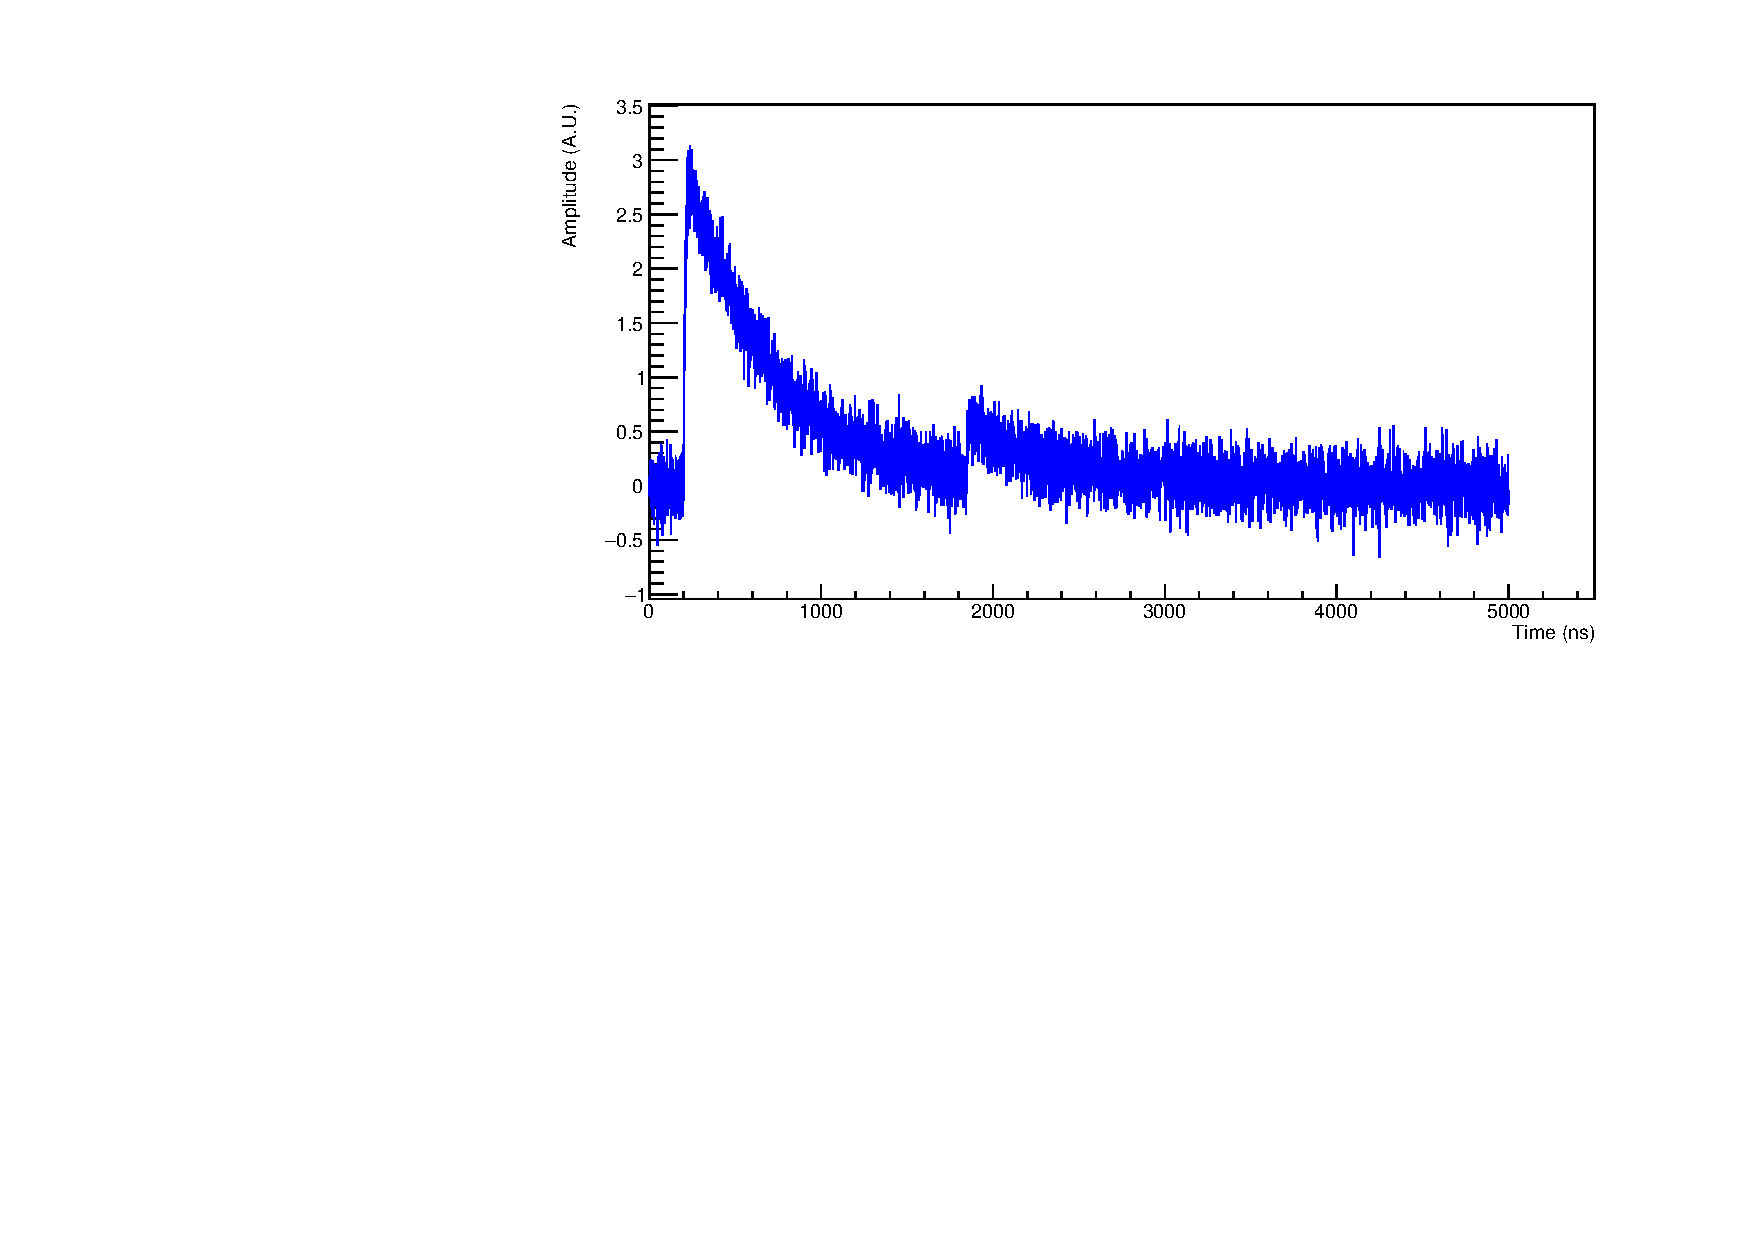
\includegraphics[width=0.8\textwidth]{IMG/Cap5/3ph_AP.pdf}
	\caption{Single waveforms generated in response to $3$ simultaneous photoelectrons with time of arrival of $20$ ns. A peak generated by AP noise is identified at $\simeq 180$ ns.}
	\label{fig:wf_ap}
\end{figure}

\subsection{Time studies} \label{subsec:Time}
An important aspect that has to be studied is the time evolution of the signals.
For that, data from $1000$ events have been generated. In each event a $20$ GeV electron, produced at the interaction point, showered in tower 1 of the GEANT4 DR calorimeter simulation.\\
We firstly analysed the distribution of the time of arrival of the photons converted at the SiPMs surface (i.e. the time recorded in the GEANT4 simulation output).\\
The distributions obtained for $C$ and $S$ photons are plotted in Figure \ref{fig:true_toa_dist}, where each entry corresponds to a single-photon time of arrival.
As expected, the distribution of the $C$ photon time of arrival is extremely narrow due to the prompt production of photons at the passage of relativistic charged particle in the fibres. Conversely, the $S$ photon time distribution shows an exponential tail due to the emission time constant of the polystyrene-based scintillators ($\tau = 2.8$ ns).\\

\begin{figure}
	\centering
	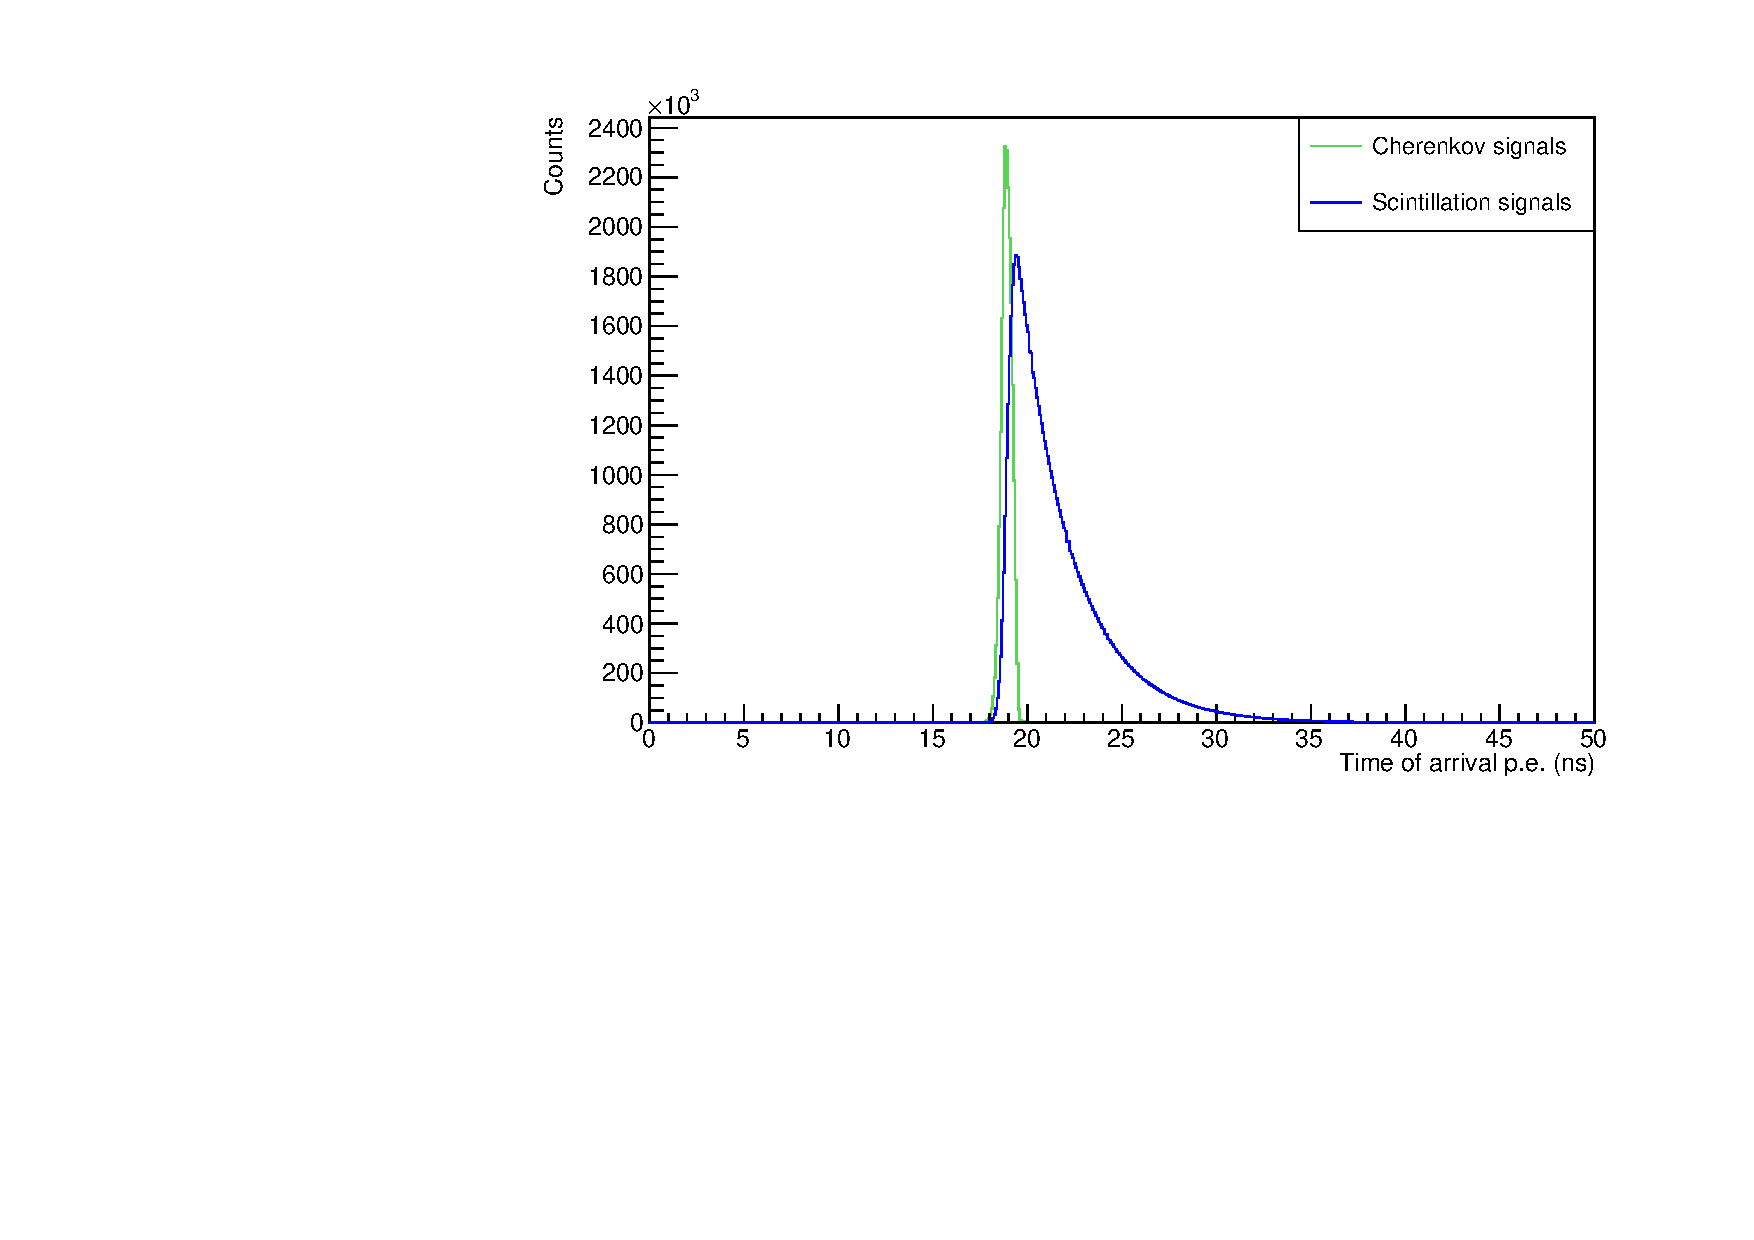
\includegraphics[width=0.85\textwidth]{IMG/Cap5/TrueTimeDist20GeV}
	\caption{The distributions of the time of arrivals of photons at the SiPMs surface, separately for Cherenkov and scintillation fibres.}
	\label{fig:true_toa_dist}
\end{figure}

These data are then used as input for \textit{pySiPM}. The SiPM parameters are chosen as described in Paragraph \ref{subsec:SiPM_conf}. In this context the most interesting parameter is the SiPM decay time constant.\\
Figures \ref{fig:top_10ns} and \ref{fig:top_50ns} show the peaking-time distributions for the two different SiPM configurations.\\
These data can be compared looking for differences as a function of the SiPM configuration.
Figure \ref{fig:top_per_fib}(a) and (b) show the peaking-time distributions for Cherenkov and scintillation signals, respectively, in the two SiPM configuration. As expected, a broadening occurs with a larger effect for the configuration with $\tau_{fall} = 50$ ns. 
In this case, the wider response function, on top of the electrical noise, causes a lost in time-of-peak resolution quantified by the broadening shown in the plots.\\

\begin{figure}
	\centering
	\subfloat[][\label{fig:top_10ns}$\tau_{fall} = 10$ ns.]{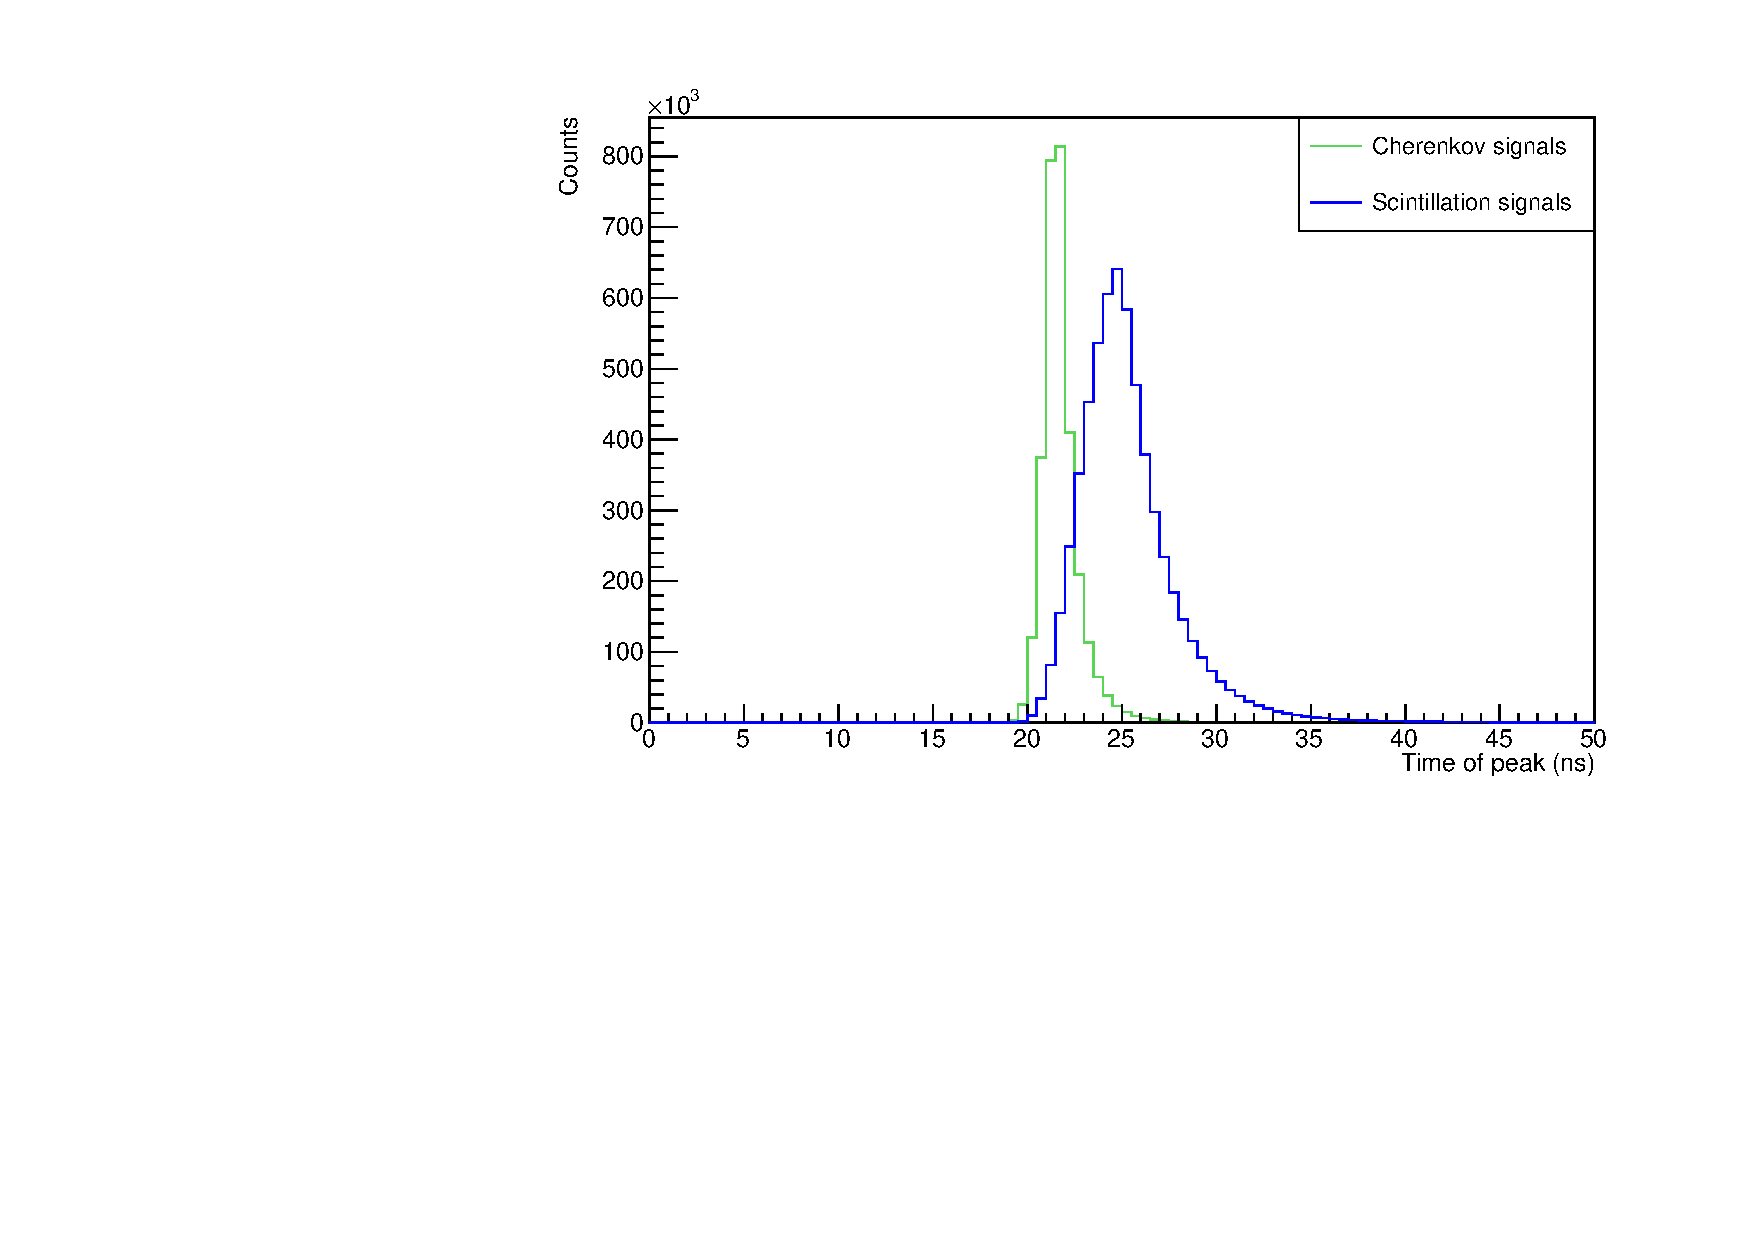
\includegraphics[width=.85\textwidth]{IMG/Cap5/ToP_20GeV_10ns}} \quad
	\subfloat[][\label{fig:top_50ns}$\tau_{fall} = 50$ ns.]{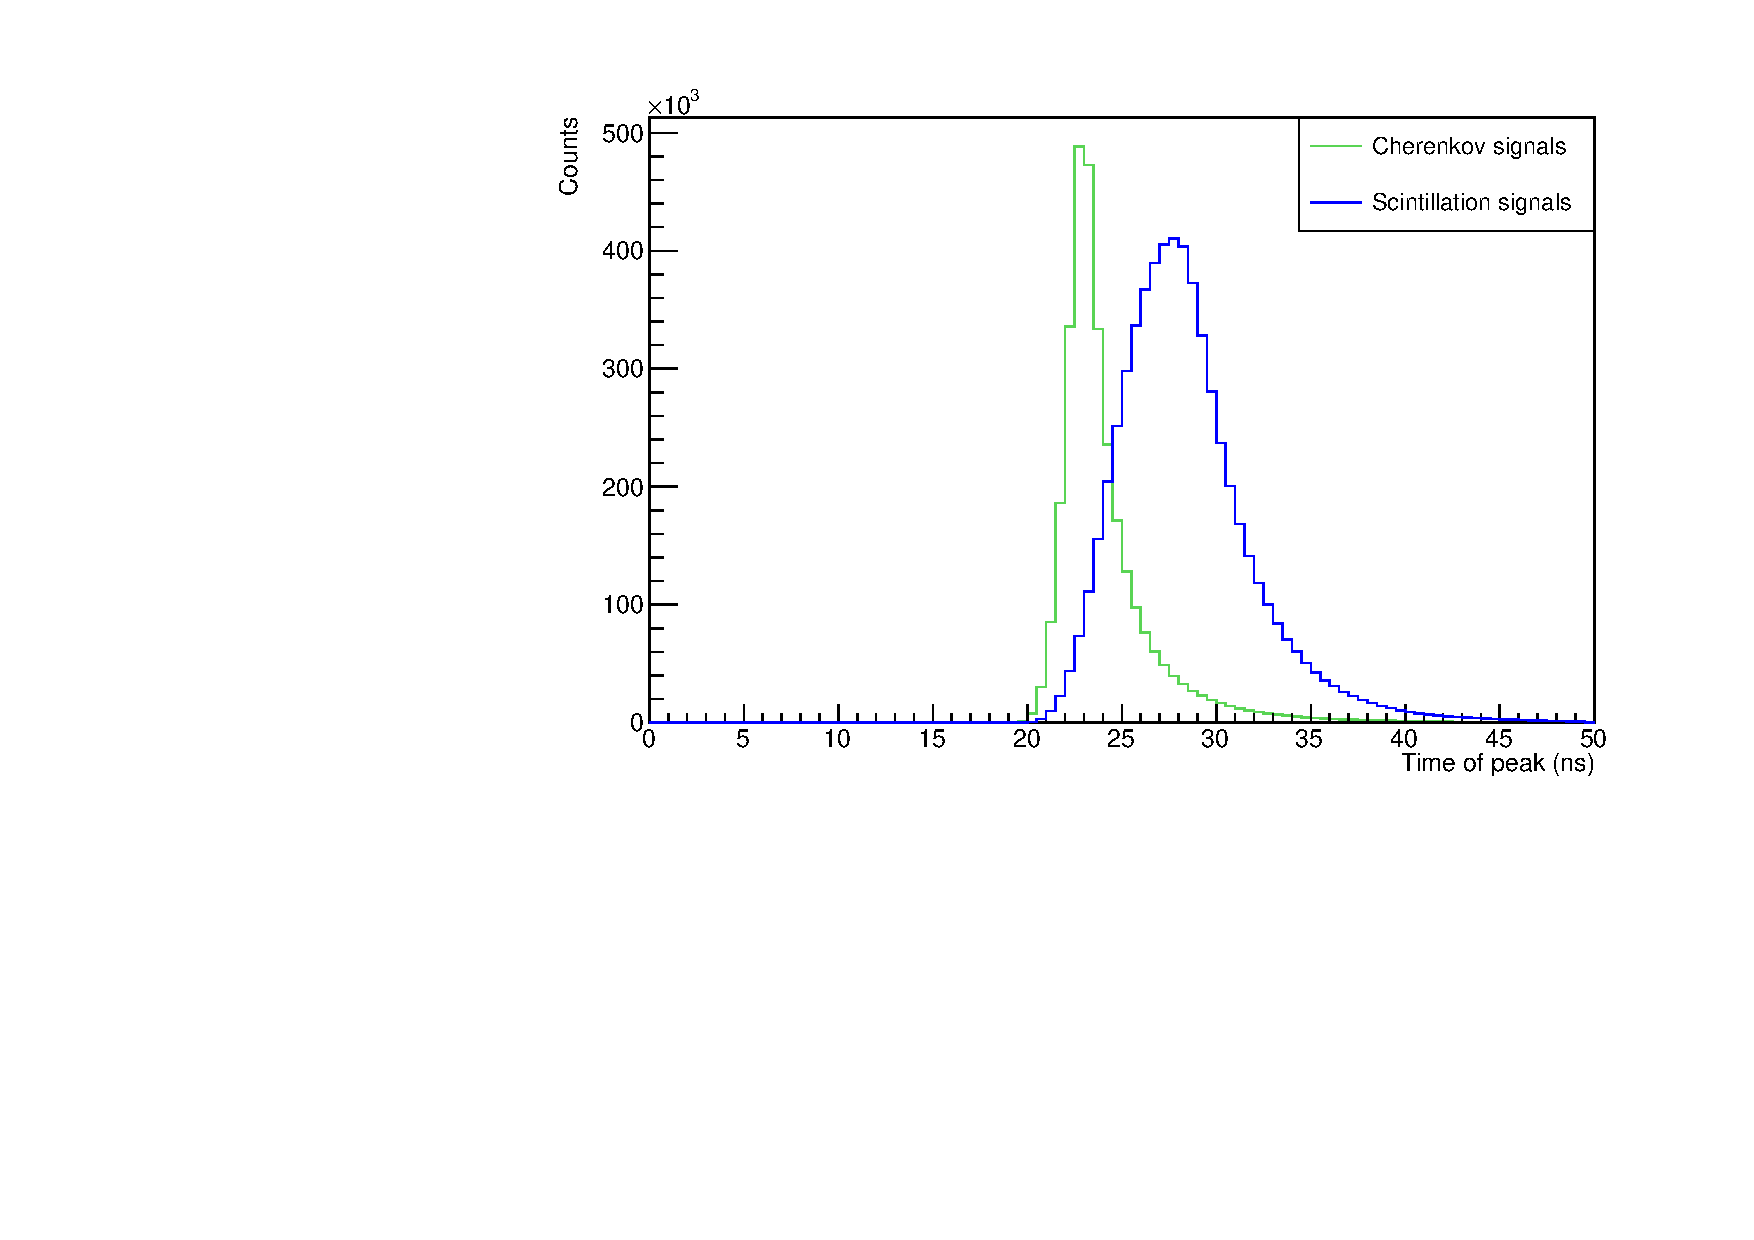
\includegraphics[width=.85\textwidth]{IMG/Cap5/ToP_20GeV_50ns}}
	\caption{Time-of-peak distributions comparing in each histogram the signals for Cherenkov and for scintillation fibres. Different figures correspond to different decay time constants. Results for $20$ GeV electrons.}
	\label{fig:top_per_tau}
\end{figure}

\begin{figure}
	\centering
	\subfloat[][\label{fig:top_C}Cherenkov fibres.]{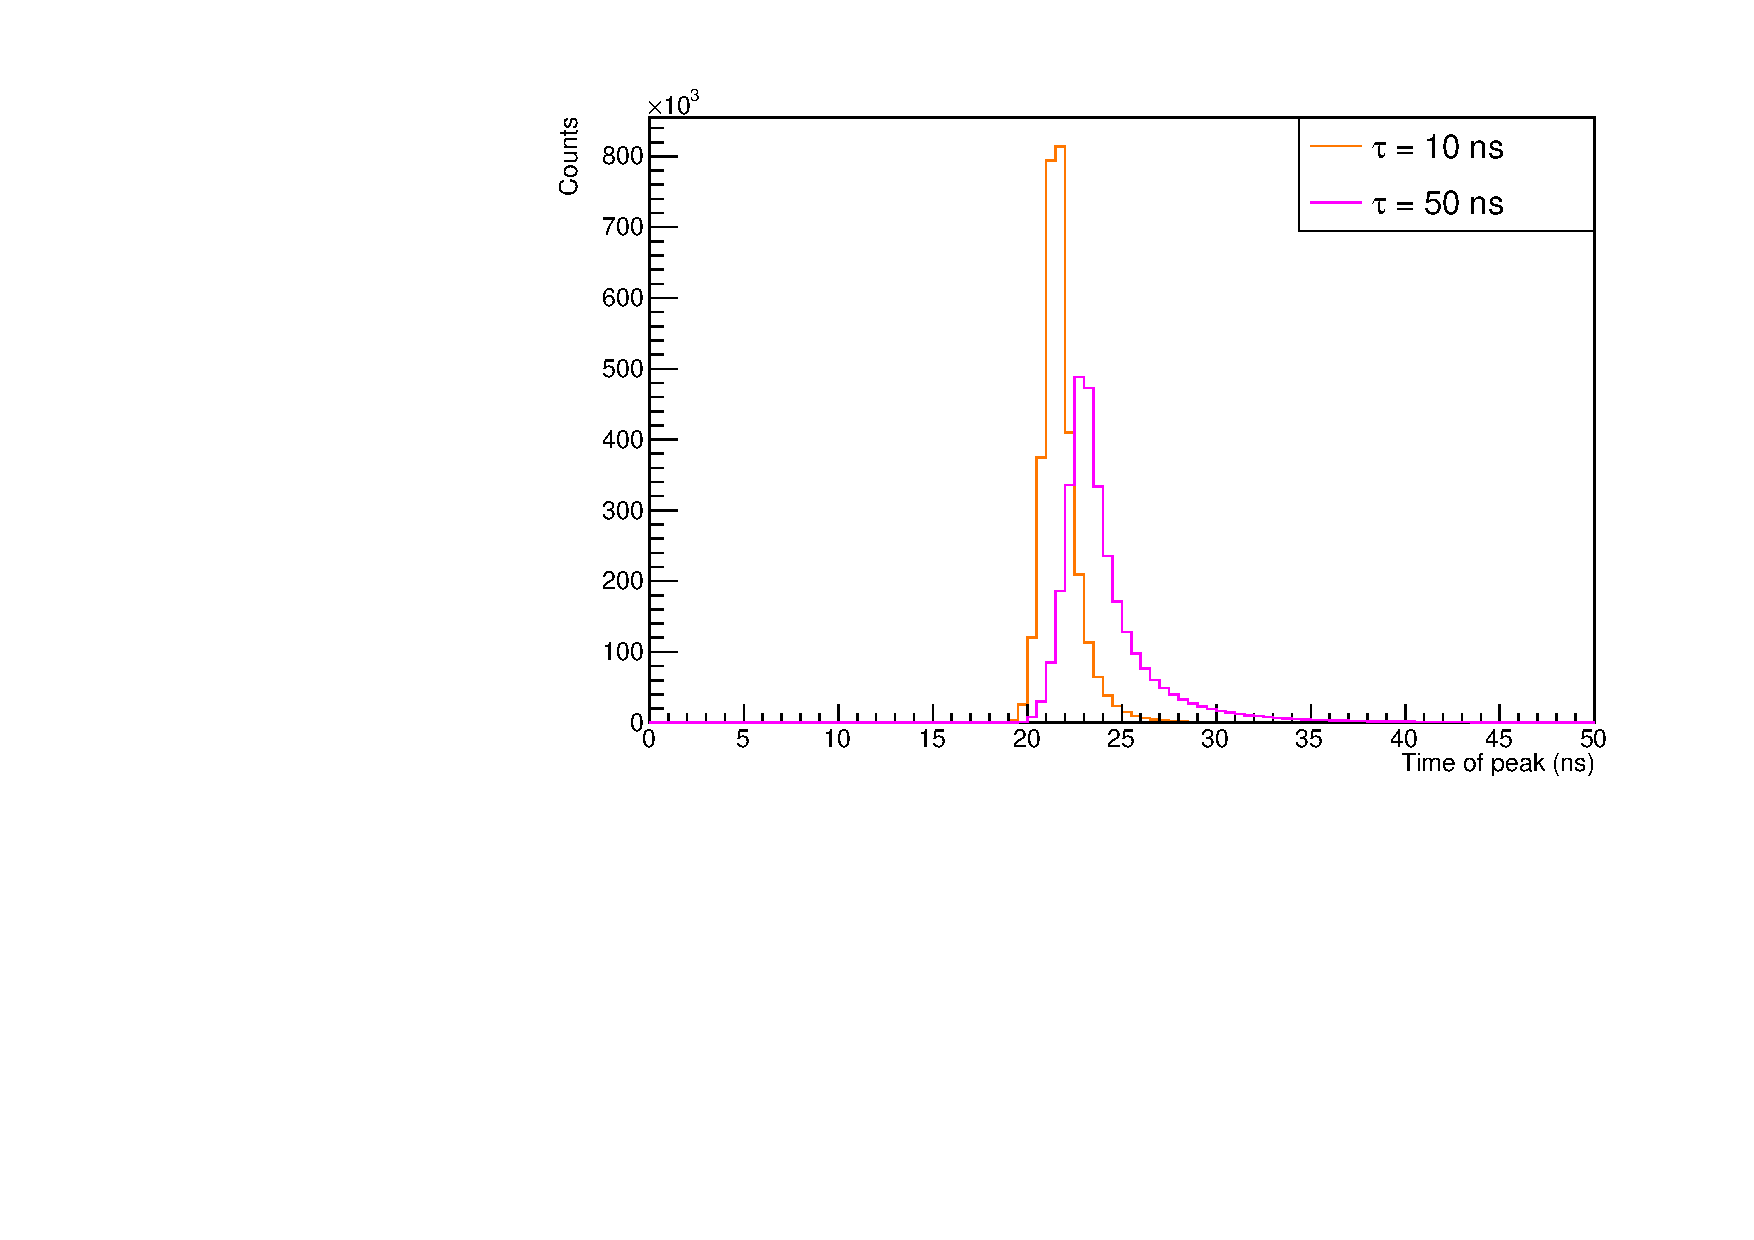
\includegraphics[width=.85\textwidth]{IMG/Cap5/ToP_20GeV_cher}} \quad
	\subfloat[][\label{fig:top_S}Scintillation fibres.]{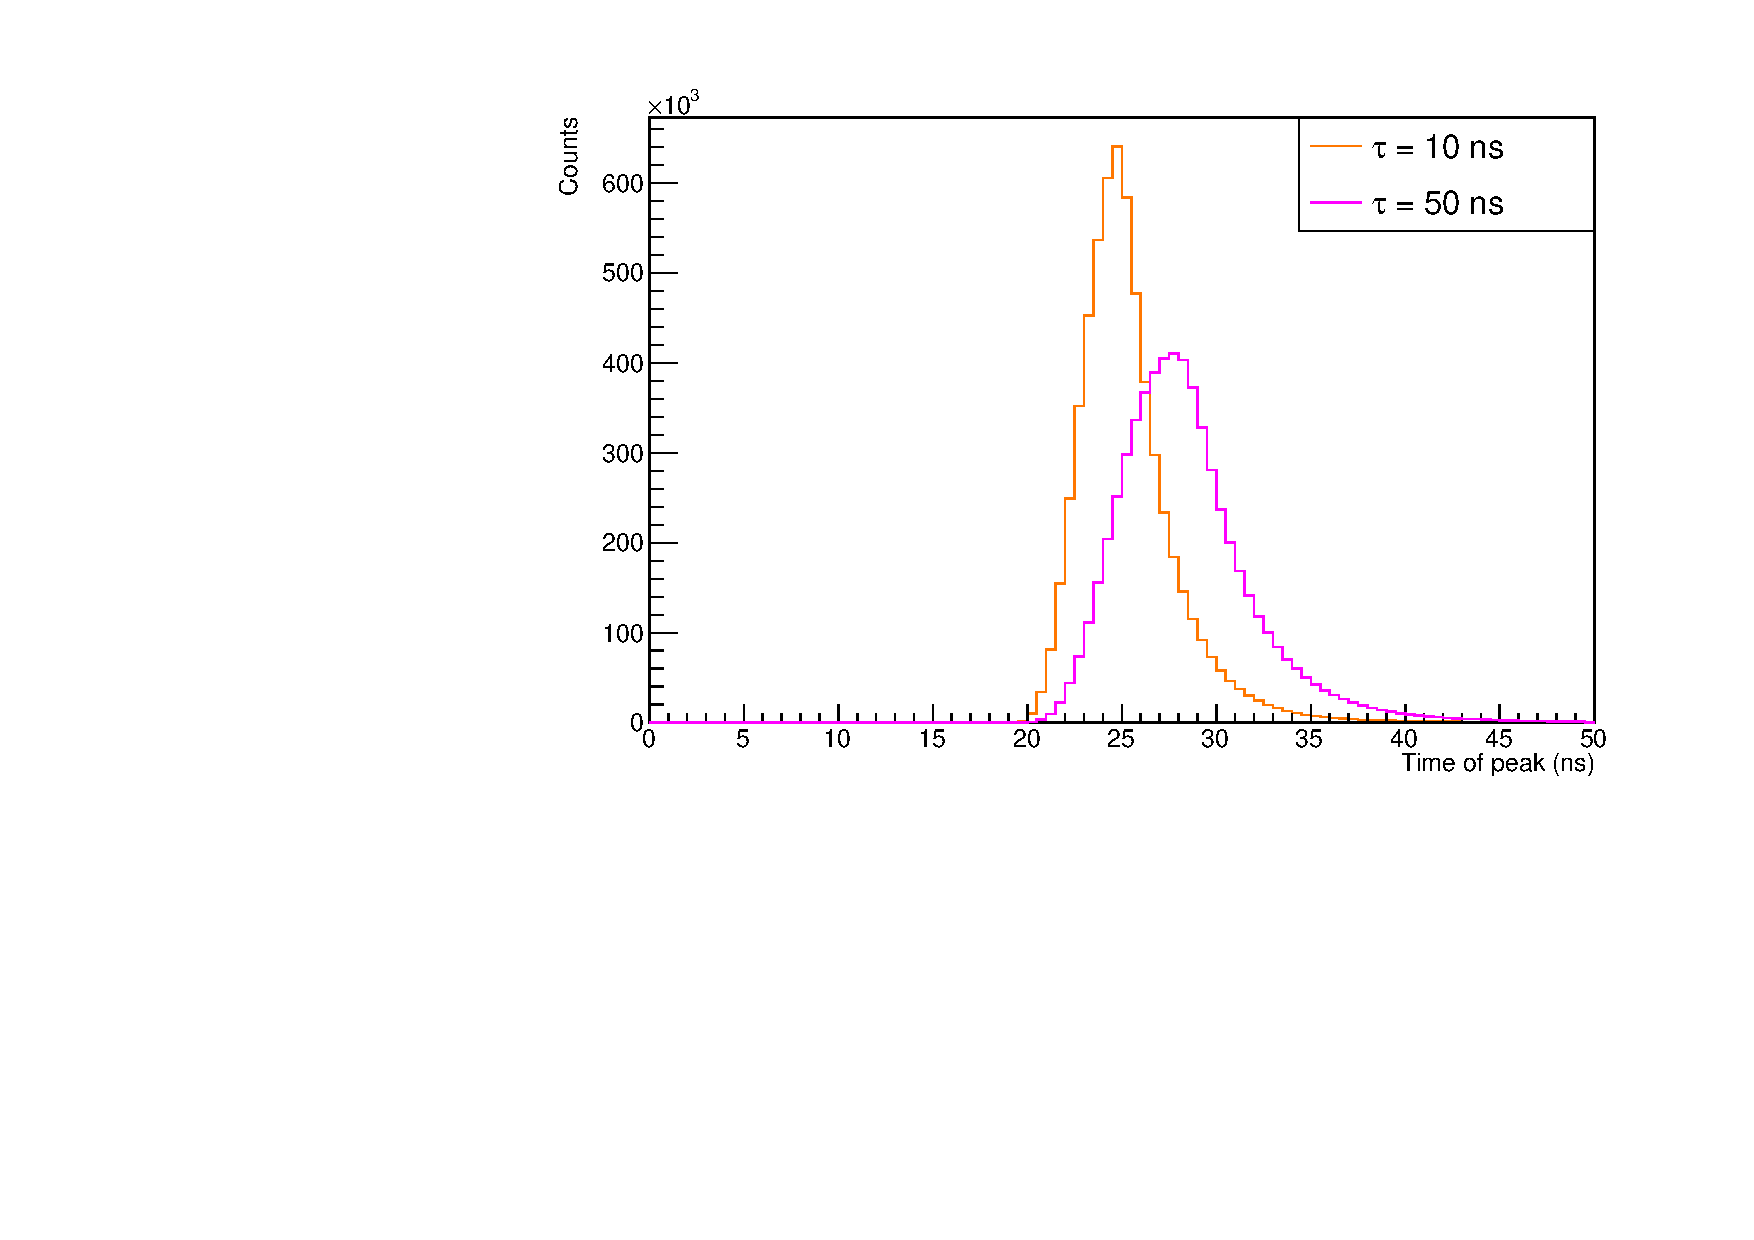
\includegraphics[width=.85\textwidth]{IMG/Cap5/ToP_20GeV_scin}}
	\caption{Time-of-peak distributions comparing in each histogram, the signals generated with two different SiPM decay time constants, (a) for the Cherenkov, (b) for the scintillation fibres. Results for $20$ GeV electrons.}
	\label{fig:top_per_fib}
\end{figure}

The impact of noise on the time-of-peak resolution is also dependent on the total number of photons impinging on the same SiPM. In particular, the time-of-peak resolution improves with the number of photons.\\
To prove this, $10000$ SiPMs have been fired with an increasing number of simultaneous photons. For each fixed number of photons, the signal time of peak has been recorded, plotted in an histogram and fitted with a Gaussian function.\\
%An example of these histograms is shown in Figure \ref{fig:top_dummy}.\\

The standard deviation of these Gaussian fits is used as estimator for the resolution and has been recorded and reported in Table \ref{tab:sigmas}.\\
It is interesting to plot these data and study the behaviour of the standard deviation as a fuction of the number of simultaneous photons ($n$), as shown in Figure \ref{fig:top_sigma}. The distribution is well interpolated with a function of the form:
\begin{equation}
	\sigma = \frac{A}{\sqrt{n}} + B.
\end{equation}
The best estimate for the parameters is: $A = 0.8712$ ns and $B = 0.08734$ ns, for data associated to SiPMs with $\tau_{fall}=10$ ns, and $A = 1.949$ ns and $B = 0.008217$ ns, for data associated to SiPMs with $\tau_{fall}=50$ ns.

\begin{table}
	\centering
	\begin{tabular}{lcc}
		\toprule
		Number of photons	& $\sigma$ with $\tau_{fall}=10$ ns (ns) & $\sigma$ with $\tau_{fall}=50$ ns (ns)	\\
		\midrule
		$1$ 	& $1.4150$ & $7.0680$ \\
		$2$ 	& $0.8717$ & $2.6420$ \\
		$3$ 	& $0.6738$ & $1.7370$ \\
		$4$ 	& $0.5742$ & $1.3770$ \\
		$5$ 	& $0.5146$ & $1.1230$ \\
		$6$ 	& $0.4624$ & $0.9719$ \\
		$7$ 	& $0.4314$ & $0.9148$ \\
		$8$ 	& $0.3998$ & $0.8508$ \\
		$9$ 	& $0.3811$ & $0.7717$ \\
		$10$ 	& $0.3605$ & $0.7169$ \\
		$25$ 	& $0.2339$ & $0.4481$ \\
		$50$ 	& $0.1679$ & $0.3112$ \\
		$100$ 	& $0.1229$ & $0.2297$ \\
		\bottomrule
	\end{tabular}
	\caption{Standard deviations obtained through a Gaussian fit of the time-of-peak distributions under different conditions.}
	\label{tab:sigmas}
\end{table}

%\begin{figure}
%	\centering
%	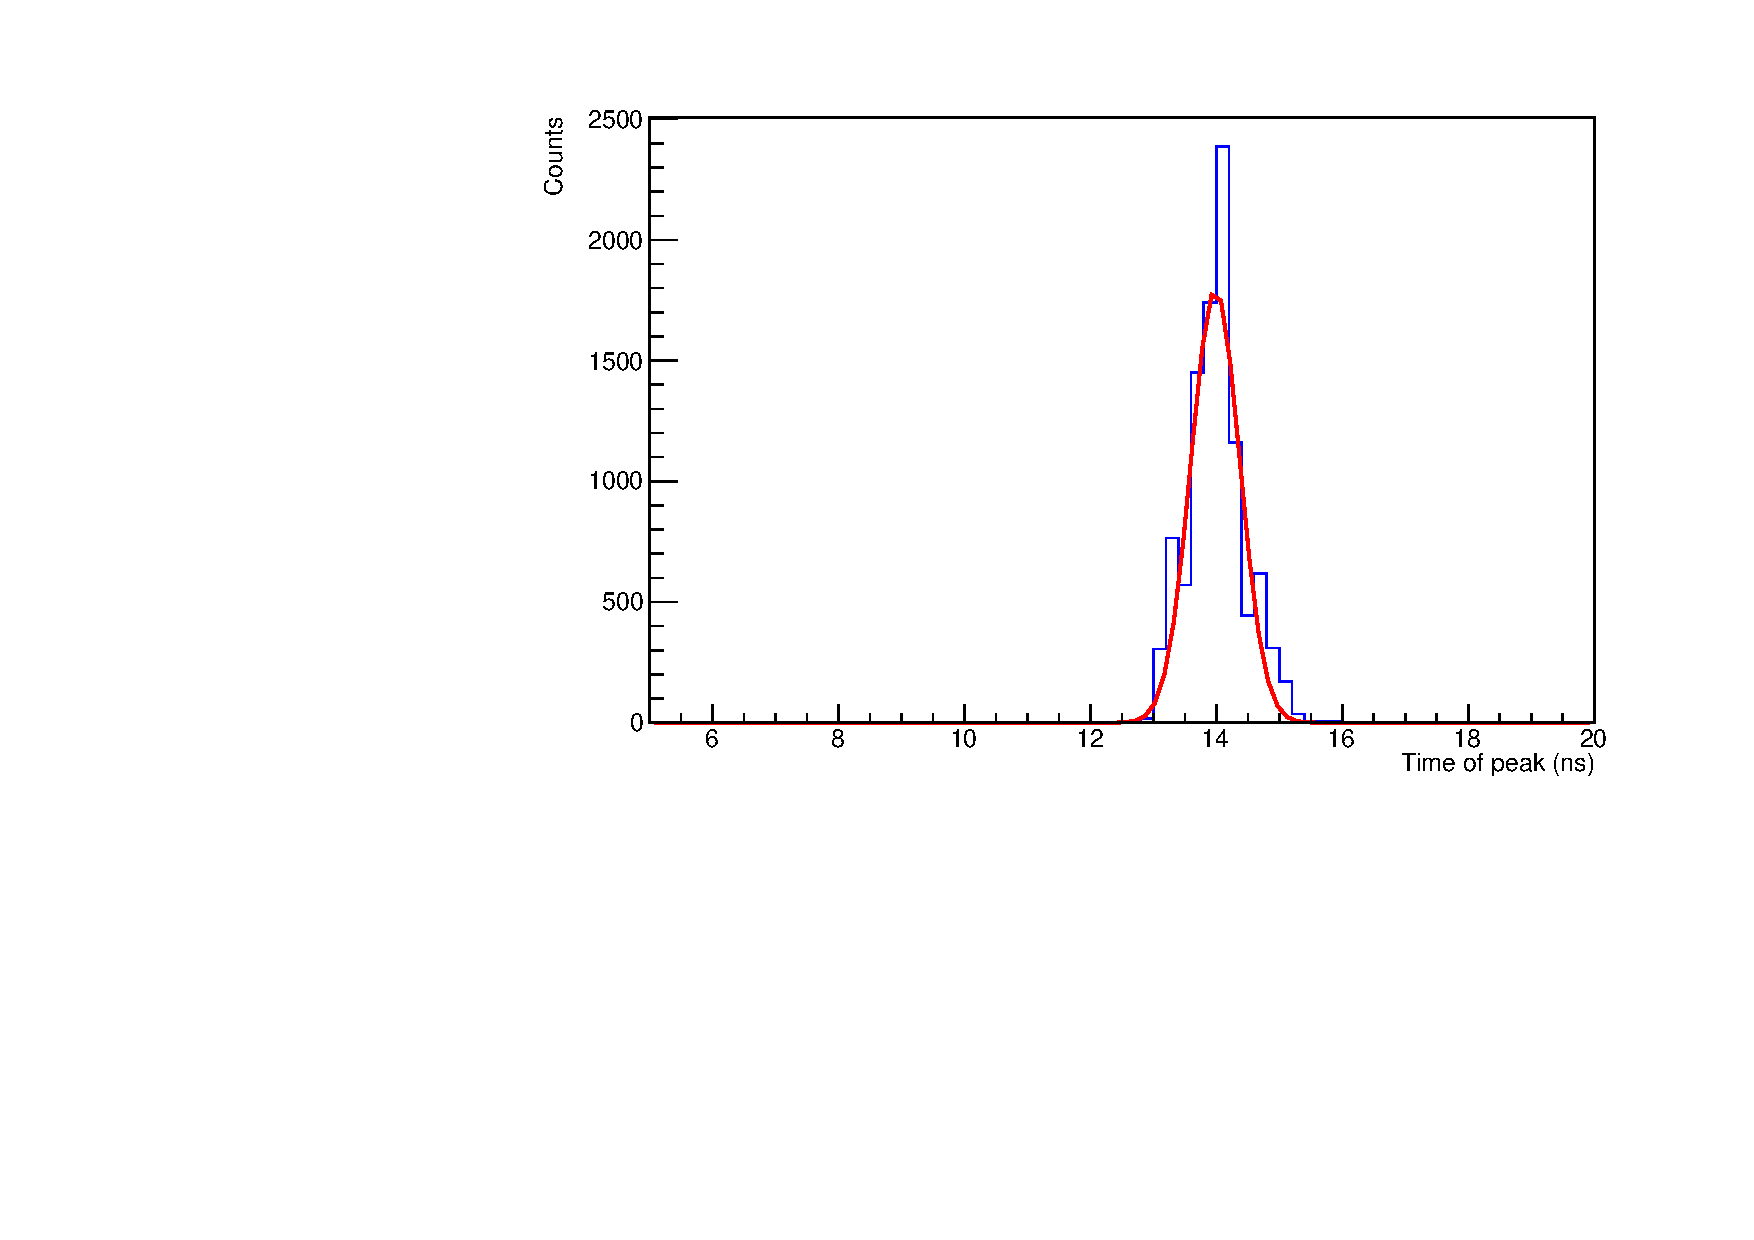
\includegraphics[width=0.85\textwidth]{IMG/Cap5/Dummy11pe_50ns}
%	\caption{Time-of-peak distribution obtained by firing $10000$ SiPMs with $11$ photoelectrons each, all reaching the SiPM surface at the same time ($10$ ns). Over this distribution a Gaussian fit has been performed.}
%	\label{fig:top_dummy}
%\end{figure}

\begin{figure}
	\centering
	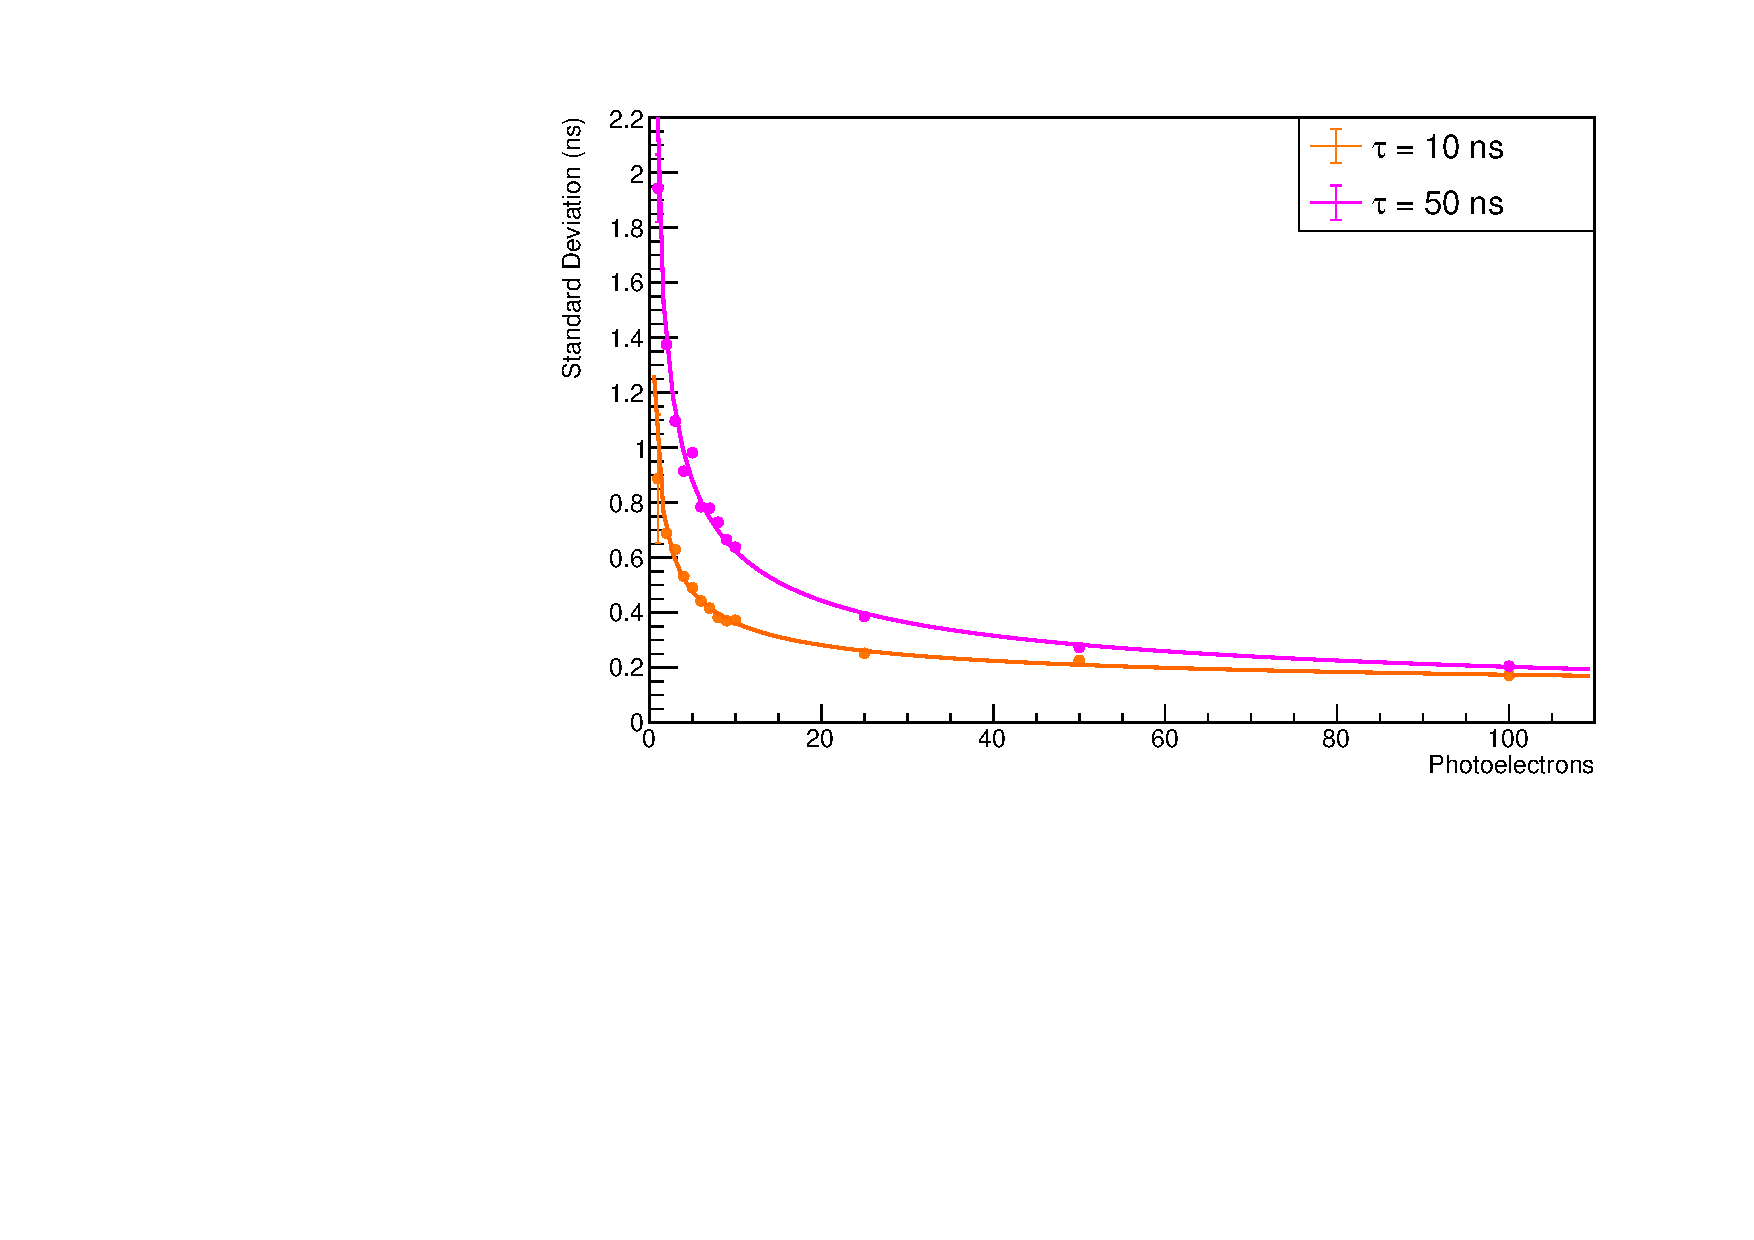
\includegraphics[width=0.85\textwidth]{IMG/Cap5/PeakSpread}
	\caption{Standard deviation of the peaking time distribution for events with a fixed number of photoelectron, as a function of the number of simultaneous photoelectrons. Study performed with two different SiPM decay-time constants.}
	\label{fig:top_sigma}
\end{figure}


\subsection{Occupancy effect} \label{subsec:Sat_effect}
The occupancy effect, described in Paragraph \ref{sec:SiPM_work}, is an important characteristic that has to be deeply studied since it may impact on the calorimeter signal linearity.\\

Figure \ref{fig:sat_example}, the charge integral as a function of the true number of p.e., shows a quantitative example:  while for small photon numbers a linear relation is found, a non-linearity effect is evident for events with many photons.\\

\begin{figure}
	\centering
	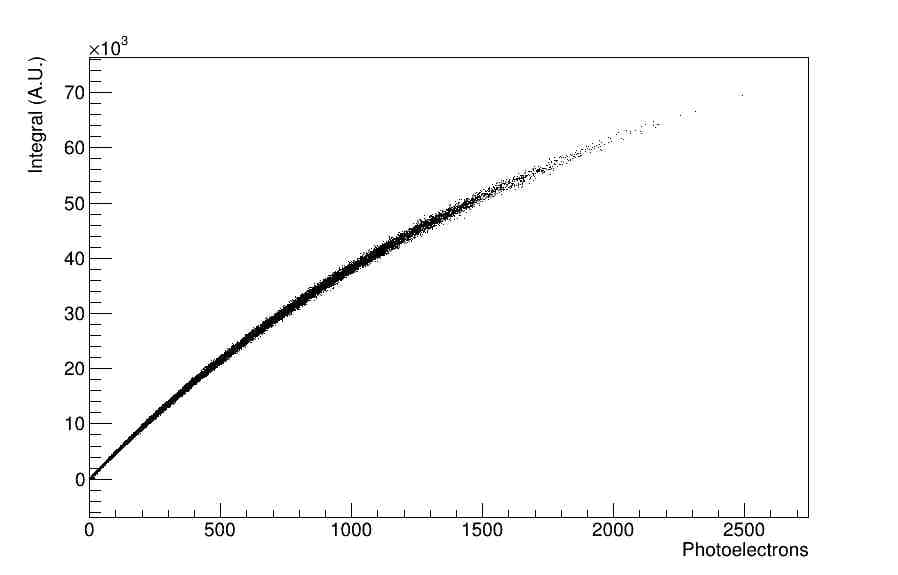
\includegraphics[width=0.85\textwidth]{IMG/Cap5/SatExample.jpg}
	\caption{Example of a (simulated) non-linearity behaviour for a SiPM with a cell size of $25$ $\mu$m.}
	\label{fig:sat_example}
\end{figure}

The simplest way to tackle this effect is to (possibly) identify a calibration analytical function that reproduces the charge integral with respect to the number of impinging p.e.\\
Starting by assuming that, in the range from $2$ to $10$ photoelectrons, in our SiPM configurations (i.e. $10000$, $4356$ or $1600$ cells in each SiPM),
%the saturation effect does not occur%
the response is linear, $10000$ SiPMs have been fired $9$ times with an increasing number of simultaneous p.e.s (from 2 up to 10).\\
As a sanity check of the above assumption, the charge integral distribution from the three different configurations has been compared and no bias was found, as shown in Figure \ref{fig:SatCheck}. The mean and the RMS values have been recorded and their behaviour with the number of photons, sketched in Figure \ref{fig:NoSatLine}, was fitted with a straight line allowing to obtain the initial calibration law:
\begin{equation}
	I(n) = A \cdot n + B
\end{equation}
with $A = 49.43 \pm 0.03852$ and $B = 2.491 \pm 0.2516$ (Fig. \ref{fig:NoSatLine}).\\
The parameter $A$ represents the contribution to the charge integral associated to a single photoelectron. Instead, $B$ is the pedestal originated mostly by the DCR events inside the integration time window. This contribution can be compared to analytical calculation.
In the simulation, we defined a DCR of $200$ kH and an integration window of $300$ ns. The pedestal contribution due to DCR can be estimated as follows:\\
$B_{DCR} = 2 \cdot 10^5 \cdot 3 \cdot 10^{-7} p.e. = 6\cdot 10^{-2} p.e. = 6\cdot 10^{-2} \cdot 49.43 = 2.96$ (in good agreement with the fit result).\\
In the following, the pedestal (fitted) value is always subtracted to the charge-integral value of each SiPM.\\

\begin{figure}
	\centering
	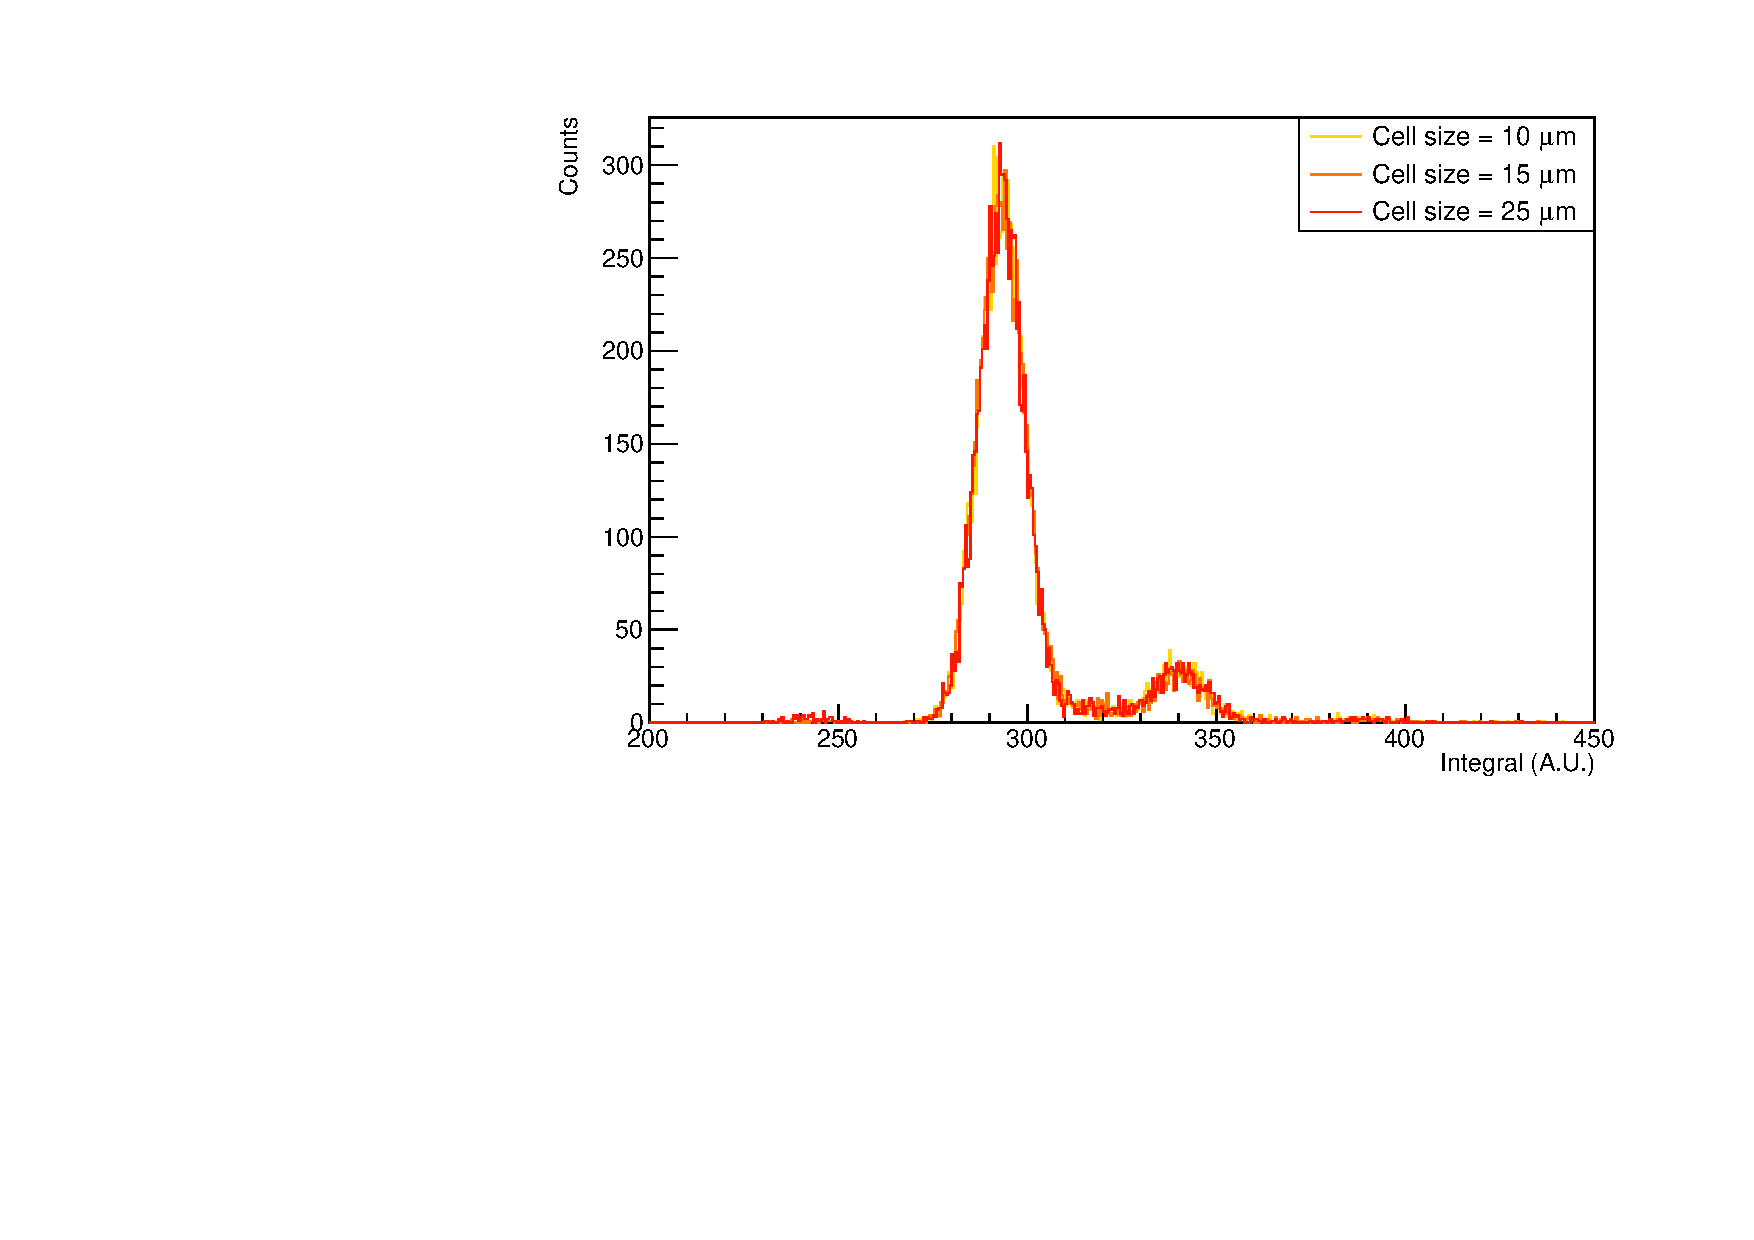
\includegraphics[width=0.85\textwidth]{IMG/Cap5/6pe_sat}
	\caption{Charge integral distributions with different SiPM cell sizes considering $6$ simultaneous photoelectrons. The distribution shape (in the full range considered, from $2$ up to $10$ simultaneous p.e.) is independent of the number of cells.
	%Results for $40$ GeV electrons.%
	}
	\label{fig:SatCheck}
\end{figure}

\begin{figure}
	\centering
	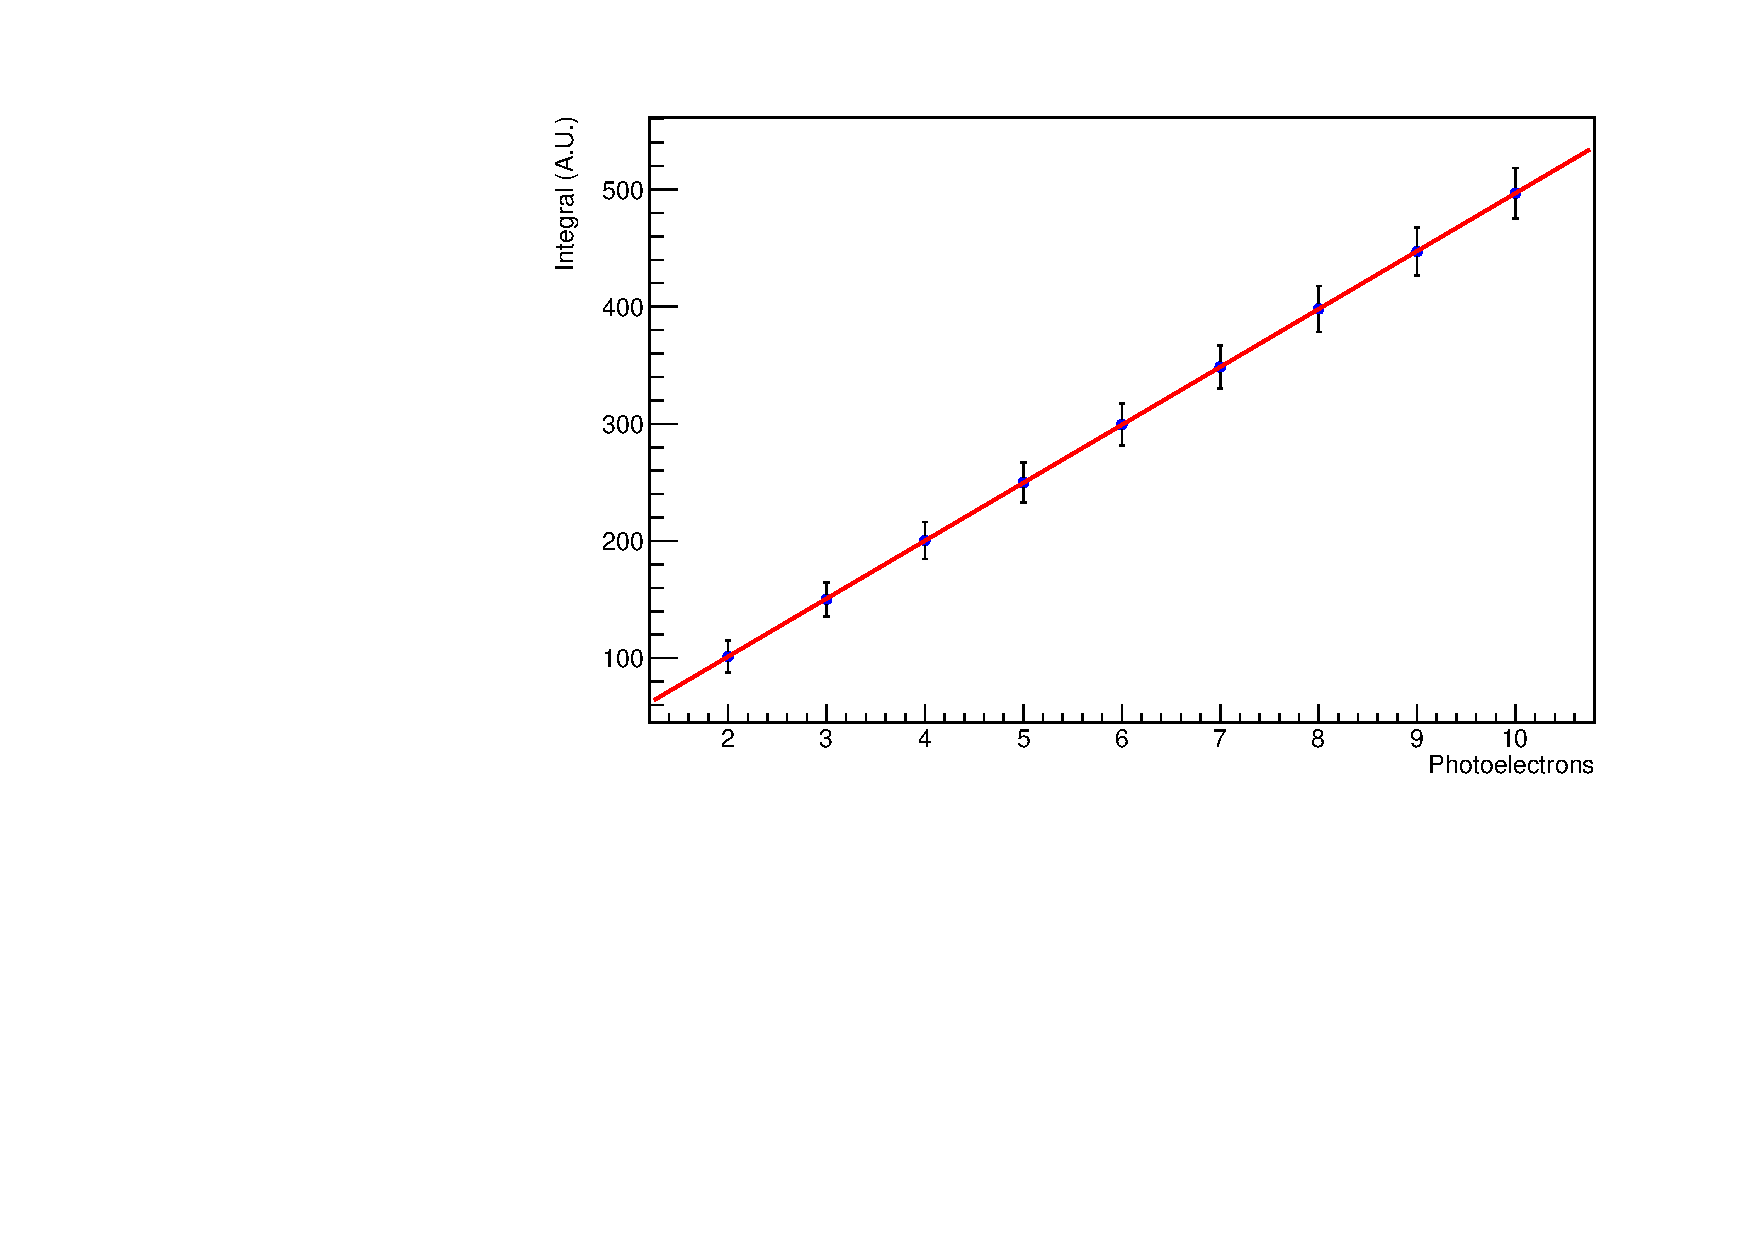
\includegraphics[width=0.85\textwidth]{IMG/Cap5/NoSatLine}
	\caption{Charge integral as a function of the number of photoelectrons, in the range from $2$ to $10$ p.e.s. A linear fit has been performed to find the calibration law in the linear regime.}
	\label{fig:NoSatLine}
\end{figure}

The occupancy effect has been studied for electromagnetic showers developing in the IDEA calorimeter simulation produced by single electrons with energies of $20,\ 40,\ 60$ and $80$ GeV.\\
The non-linearity effects have been quantified using the relation $I = A\cdot n$ (after pedestal subctraction) as reference. The results obtained with $10000$ events of single $40$ GeV $e^-$, for different SiPM configurations, are shown in Figure \ref{fig:sat_fibres}, for the Cherenkov and scintillation signals independently. For each event, there is one entry for each fibre (i.e. SiPM) that got a signal. Each point correspond to a single SiPM. Clearly, the smaller the number of cells, the greater the non-linearity effect.\\
Moreover, since, as expected, the scintillation fibres have on average $\sim 4$ times more p.e.s than the Cherenkov ones, the $S$ signal is more affected than the $C$ one.\\

\begin{figure}
	\centering
	\subfloat[][Cherenkov signals.]{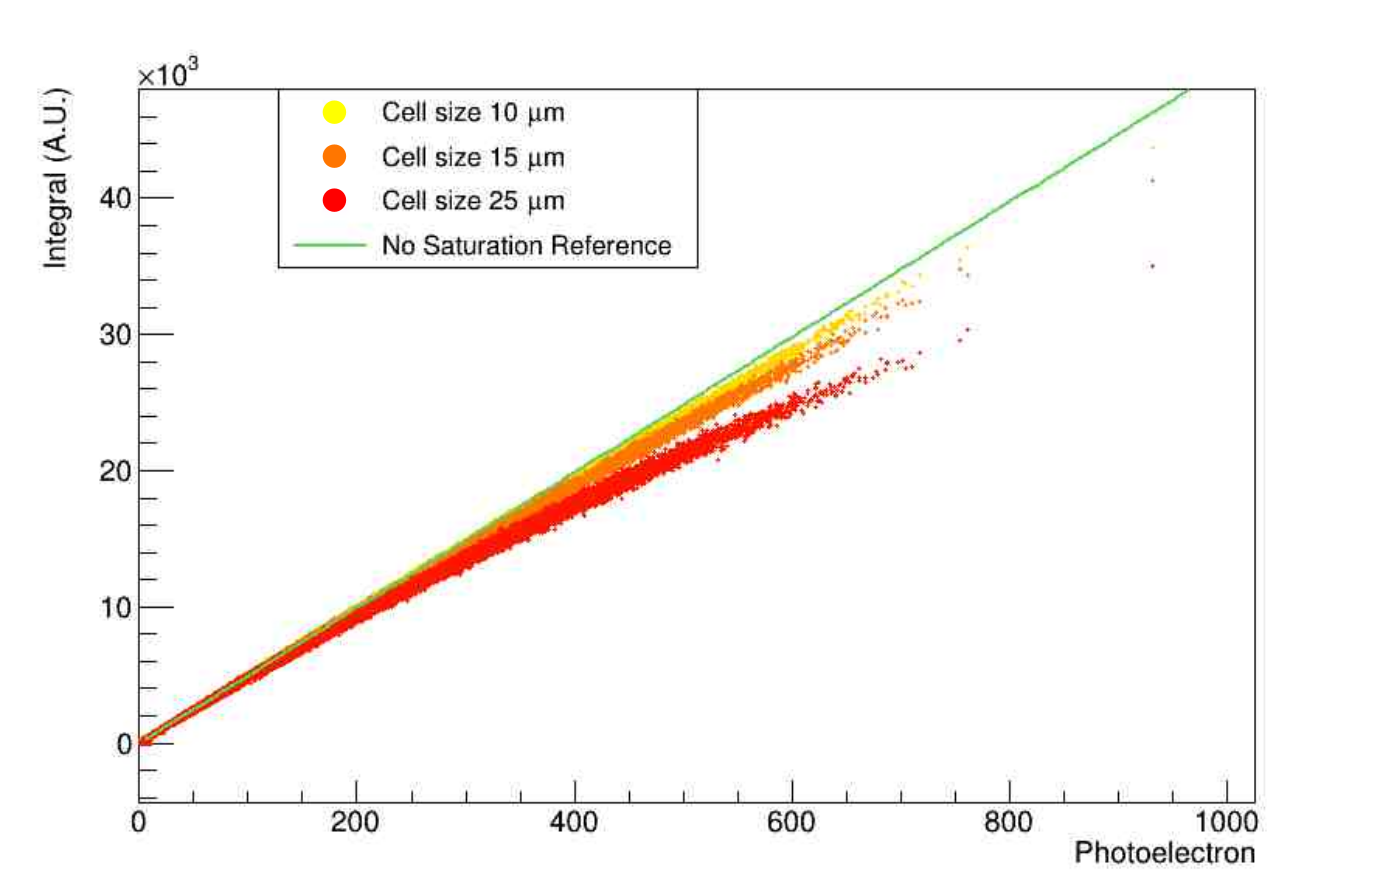
\includegraphics[width=.85\textwidth]{IMG/Cap5/Sat_Fib_40GeV_cher_dots.png}} \\
	\subfloat[][Scintillation signals.]{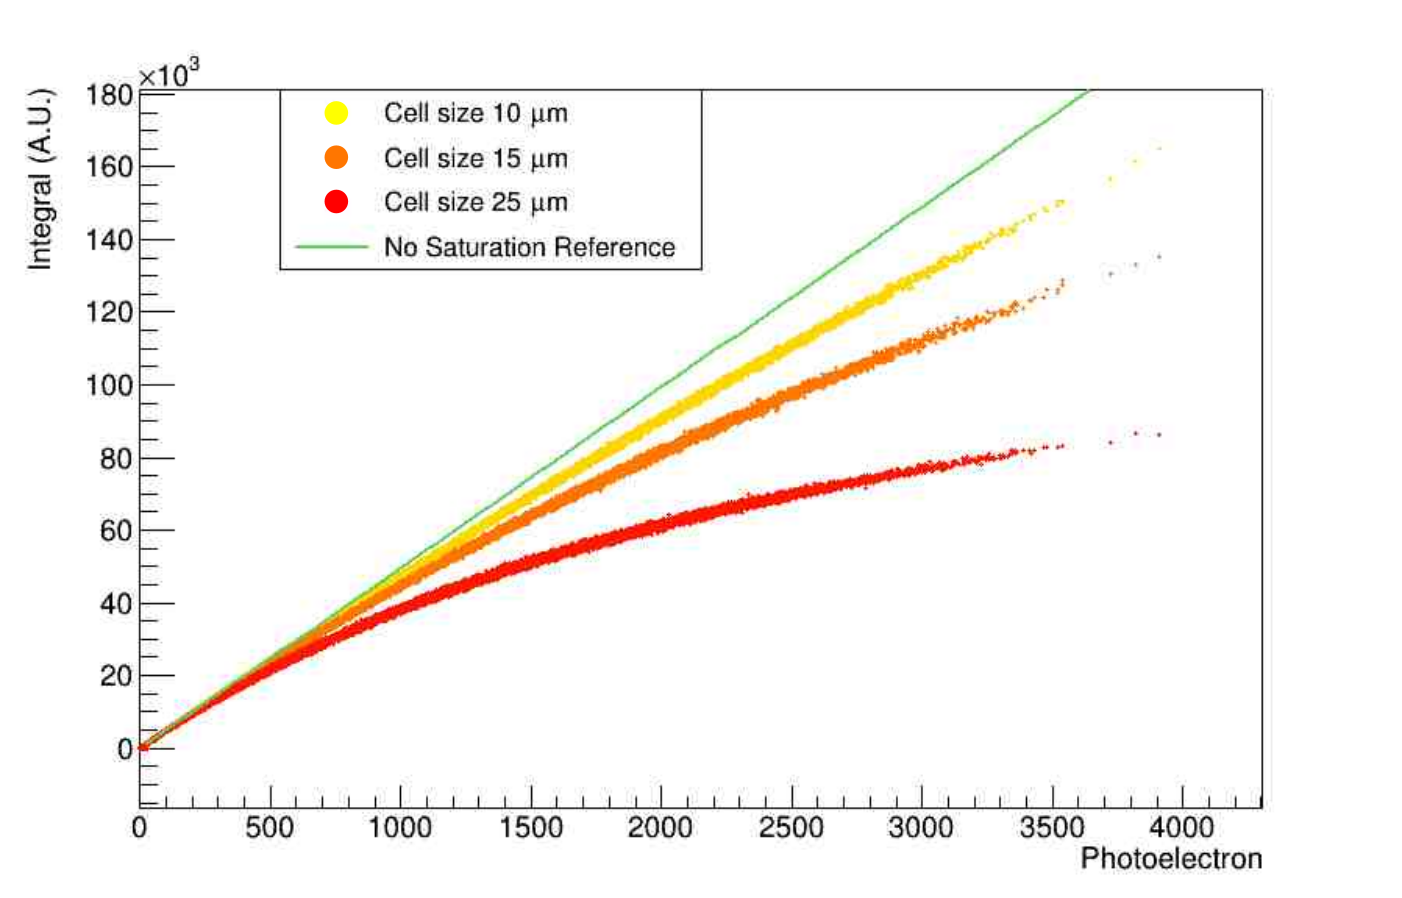
\includegraphics[width=.85\textwidth]{IMG/Cap5/Sat_Fib_40GeV_scin_dots.png}}
	\caption{The plots, (a) for the Cherenkov and (b) for the scintillation signal, show the impact of non-linearity effects for single $40$ GeV electrons, with different SiPM cell sizes. For each event, there is one entry for each fibre (i.e. SiPM) that got a signal.
	Each point corresponds to a SiPM with different values of cell size.
	The linear behaviour, as extrapolated from the fit to the plot in Figure \ref{fig:NoSatLine}, is included as reference.}
	\label{fig:sat_fibres}
\end{figure}

This process can be extended by independently integrating, the number of photoelectrons and the charge, over the full event. The result is represented in Figure \ref{fig:sat_events} where each point correspond to a single event.\\

\begin{figure}
	\centering
	\subfloat[][Cherenkov signals.]{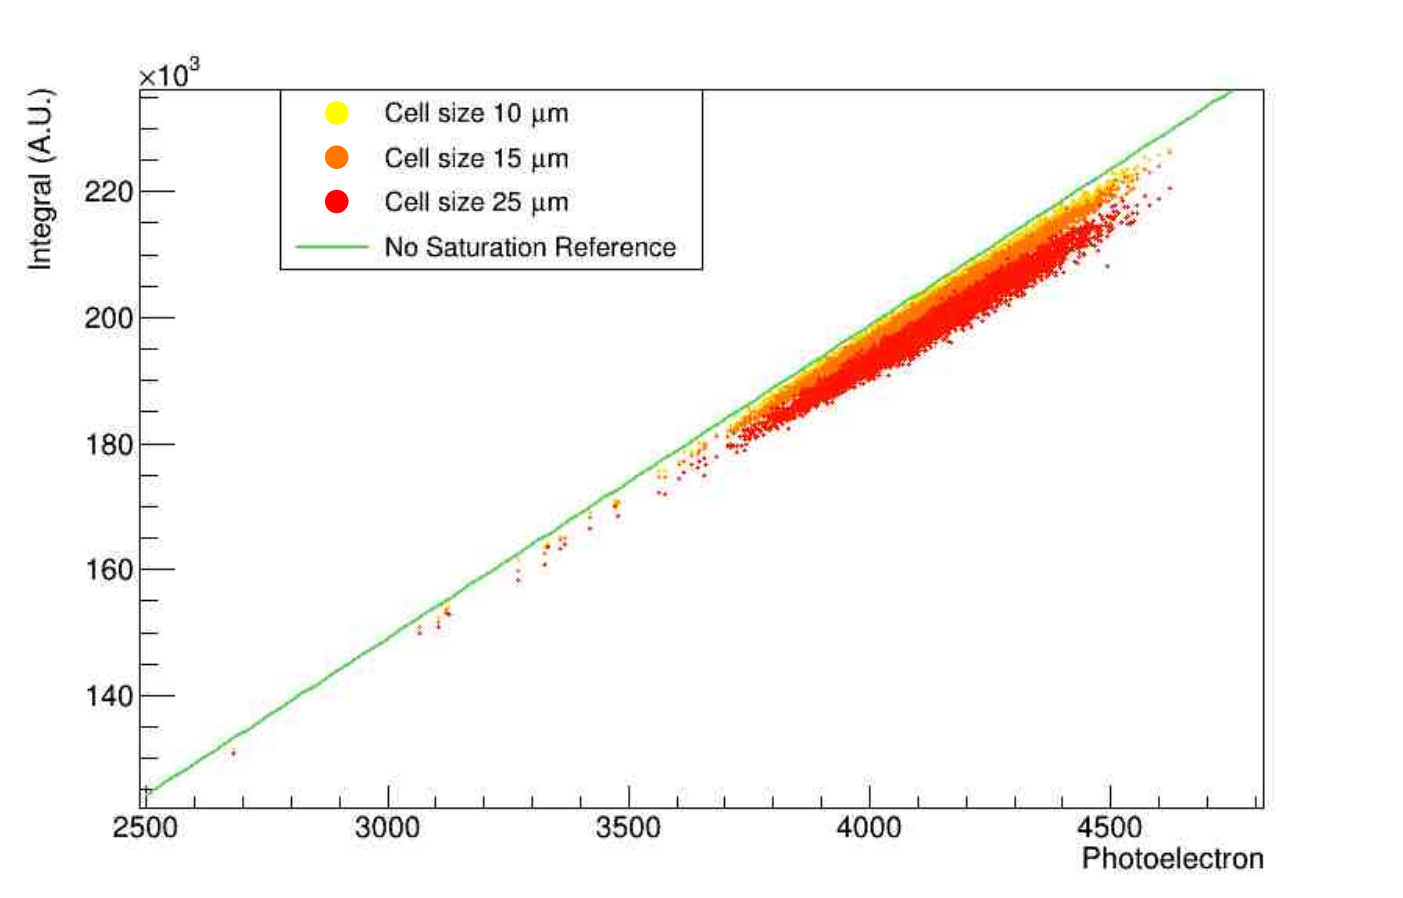
\includegraphics[width=.85\textwidth]{IMG/Cap5/Sat_Ev_40GeV_cher_dots.png}}\\
	\subfloat[][Scintillation signals.]{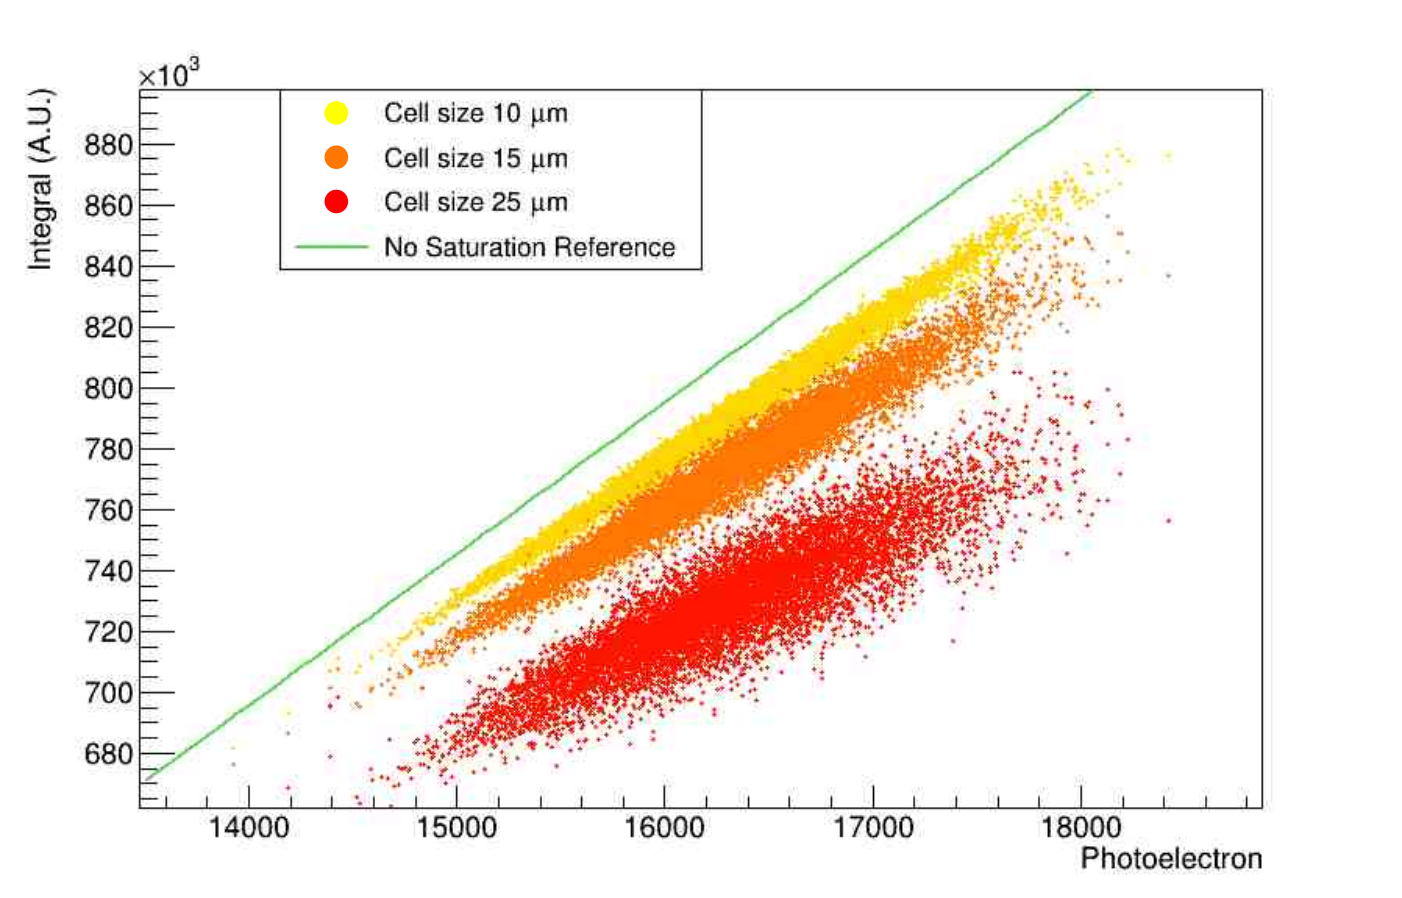
\includegraphics[width=.85\textwidth]{IMG/Cap5/Sat_Ev_40GeV_scin_dots.png}}
	\caption{The plots, (a) for the Cherenkov, (b) for the scintillation signal, show the non-linearity effects with single $40$ GeV electrons. Each of the $10000$ points correspond to a single event where the charge and the number of photoelectrons was integrated over all the fired fibres. Different values of the SiPM cell size are represented with different colours. The linear behaviour, as extrapolated from the fit to the plot in Figure \ref{fig:NoSatLine}, is included for reference.}
	\label{fig:sat_events}
\end{figure}

As can be seen, non-linearity effects show up even for $10$ $\mu$m cell SiPMs. To mitigate this problem, an analytical correction can be introduced via the formula:
\begin{equation}
	N_{fired}=N_{cells} \cdot \left[ 1 - \exp\left(-\frac{N_{p.e.}}{N_{cells}}\right)\right],
\end{equation}

The above correction has been applied by modifying the integral values as follows:
\begin{equation}
	Q_{corr} = - A N_{cells} \left[ \ln\left(1 - \frac{Q}{A N_{cells}}\right) \right],
\end{equation}
where the linear relation to convert $N_{cells}$ ($N_{fired}$) to the corresponding integral value $Q_{corr}$ ($Q$), through the constant $A$ (as fitted in the linear regime region), has been applied.

The results obtained can be found in Figures \ref{fig:sat_corr1} and \ref{fig:sat_corr2} where the data, for SiPMs with a cell size of $10$ $\mu$m, are compared with and without the analytical correction.

\begin{figure}
	\centering
	\subfloat[][Cherenkov signals. Points are single SiPMs.]{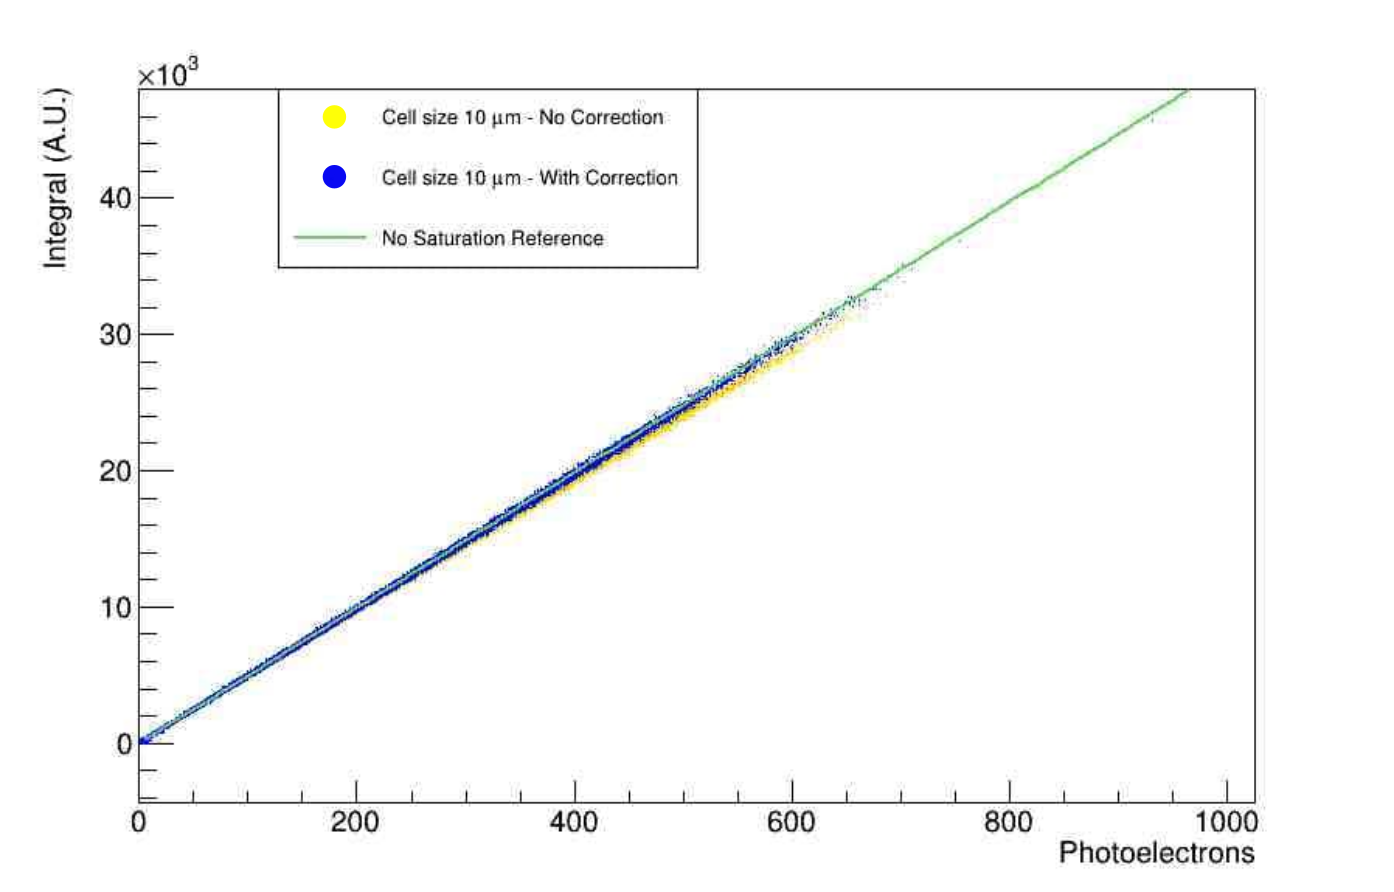
\includegraphics[width=.85\textwidth]{IMG/Cap5/SatCorr_40GeV_fib_cher_dots.png}}\quad
	\subfloat[][Scintillation signals. Points are single SiPMs.]{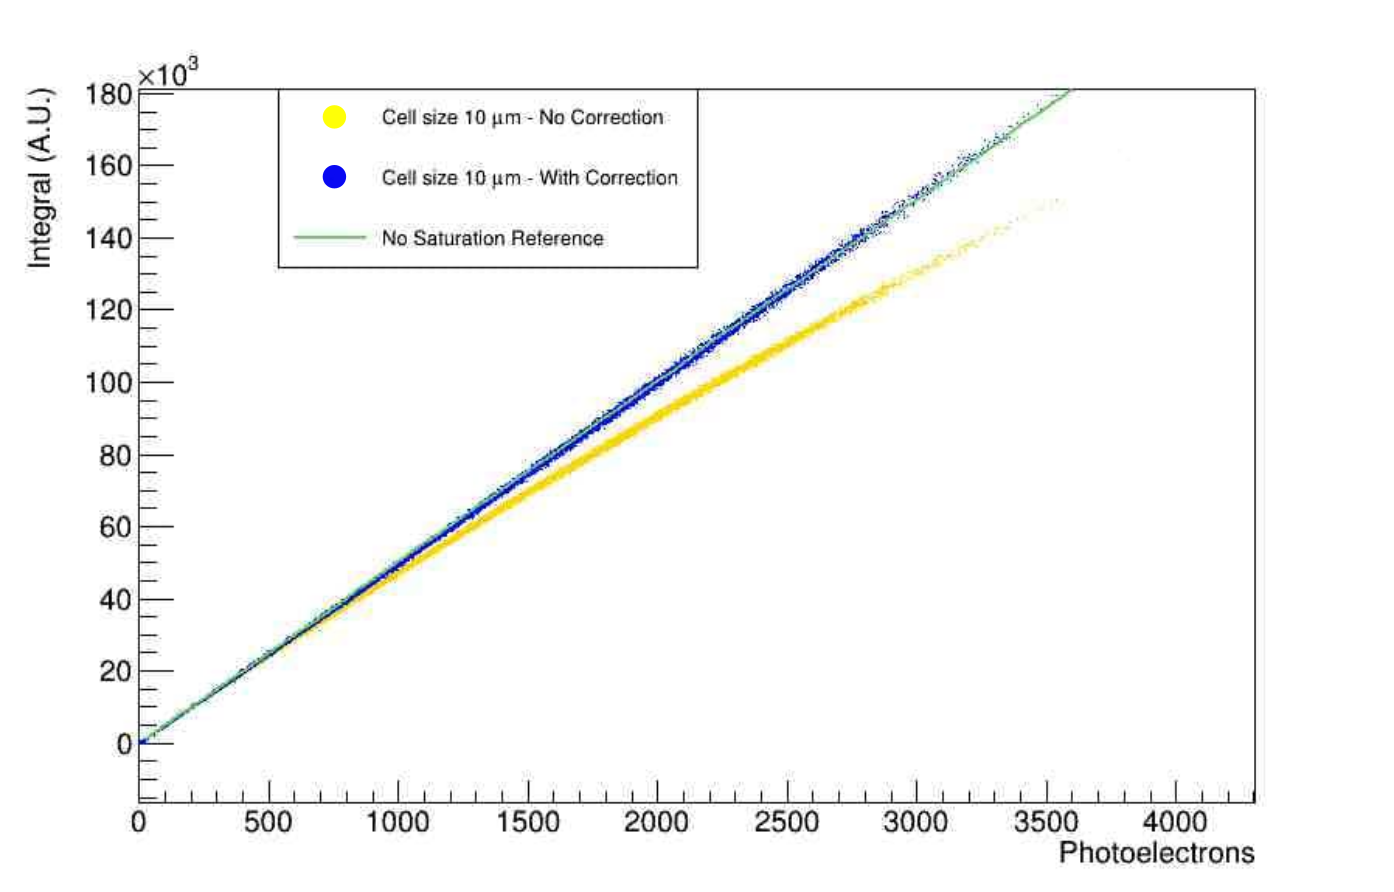
\includegraphics[width=.85\textwidth]{IMG/Cap5/SatCorr_40GeV_fib_scin_dots.png}}\\
	\caption{Similar plots to Figures \ref{fig:sat_fibres}. Each point correspond to a $10~\mu$m cell-size SiPM, with or without applying the analytical correction. Two series of data are presented to show the effectiveness of the analytical correction. The linear behaviour, as extrapolated from the fit to the plot in Figure \ref{fig:NoSatLine}, is included as reference. Results for $40$ GeV electrons.}
	\label{fig:sat_corr1}
\end{figure}

\begin{figure}
	\centering
	\subfloat[][Cherenkov signals. Points are single events.]{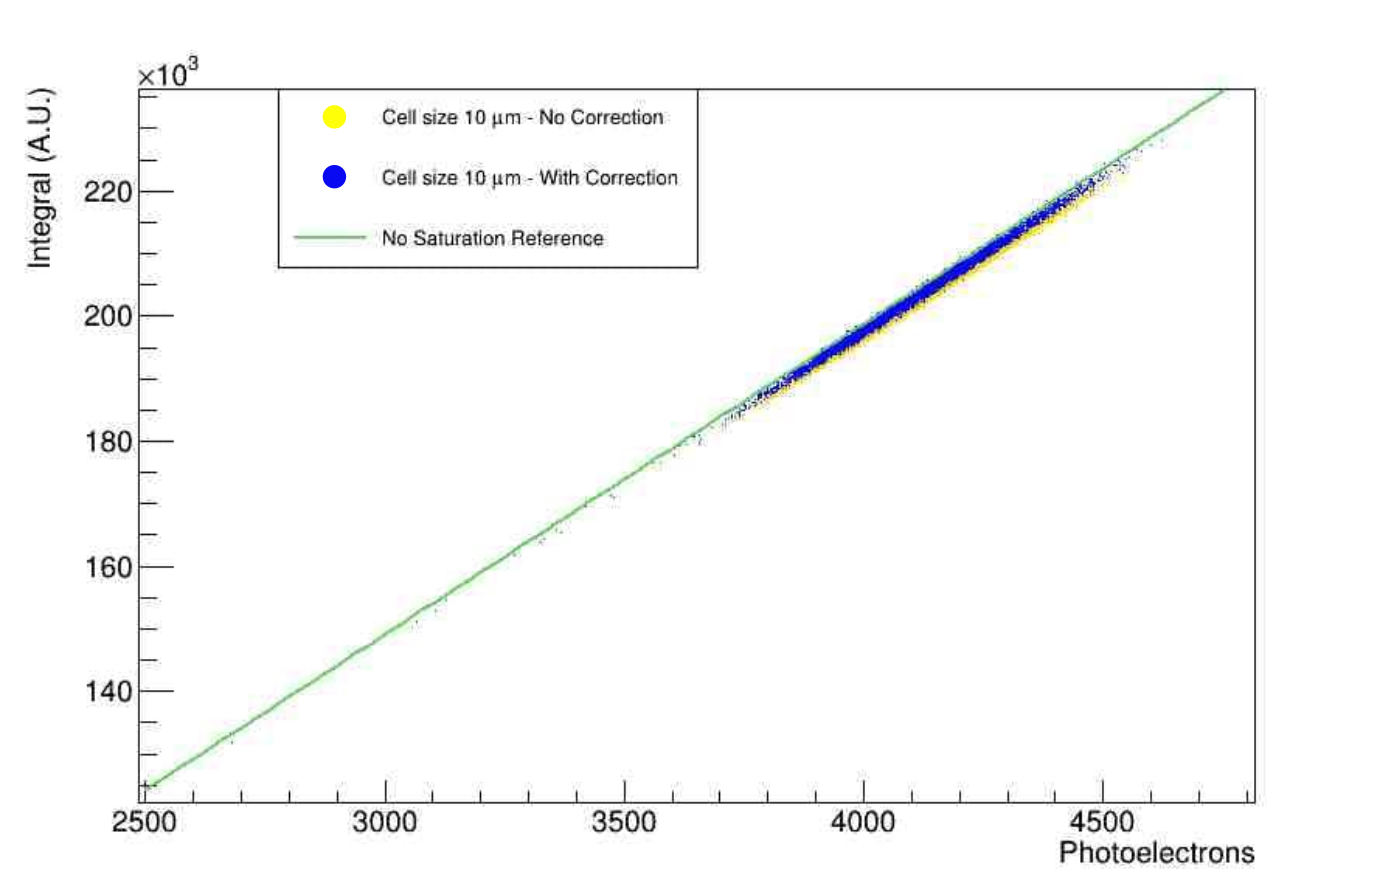
\includegraphics[width=.85\textwidth]{IMG/Cap5/SatCorr_40GeV_ev_cher_dots.png}} \quad
	\subfloat[][Scintillation signals. Points are single events.]{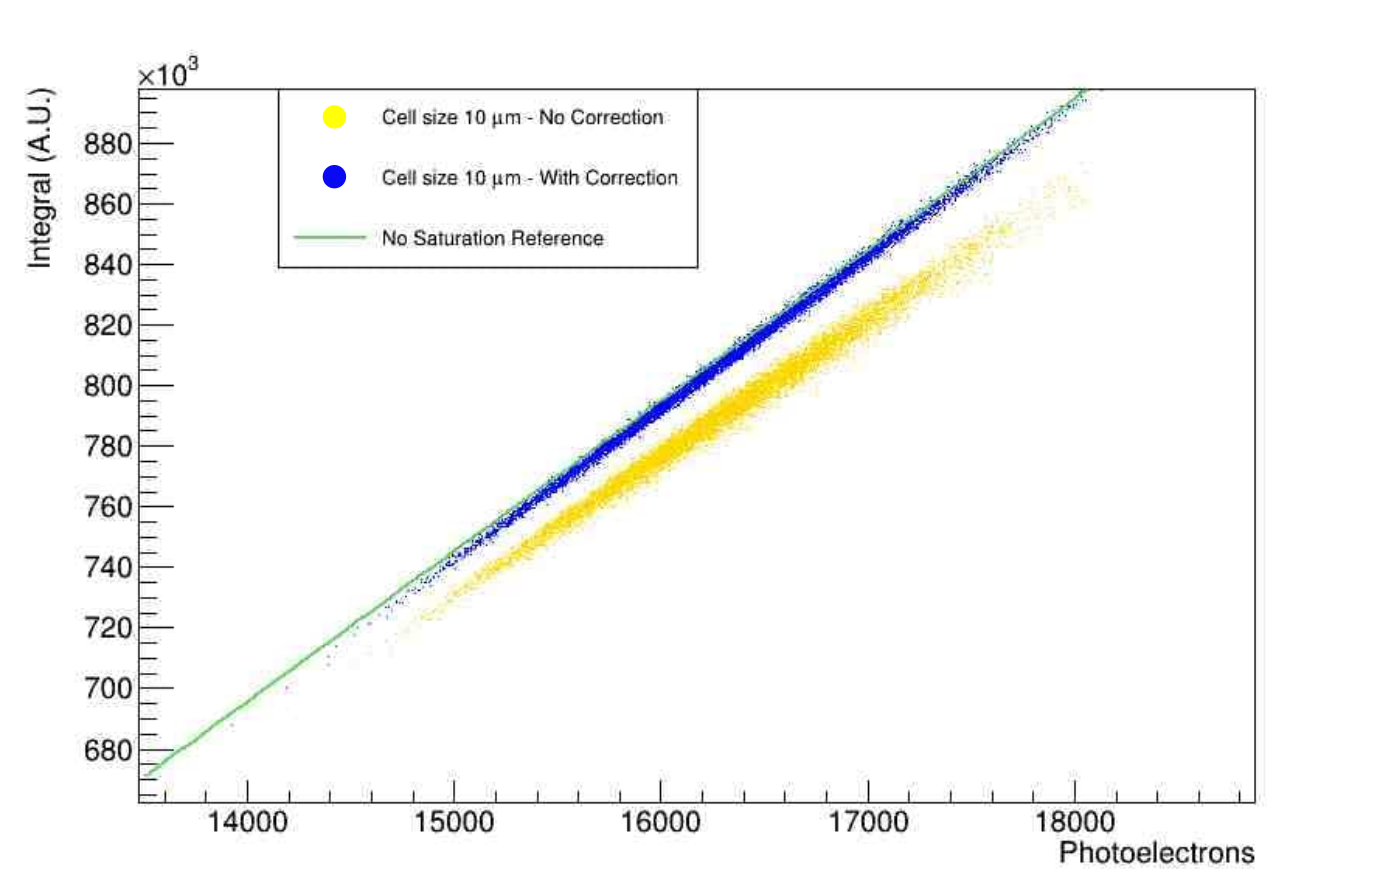
\includegraphics[width=.85\textwidth]{IMG/Cap5/SatCorr_40GeV_ev_scin_dots.png}}
	\caption{Similar plots to Figures \ref{fig:sat_events}. Each of the $10000$ points correspond to a single event where integral and number of photoelectrons have been added over the fired SiPMs. Two series of data (with or without applying the analytical correction) are presented to show the effectiveness of the analytical correction. The no saturation line shown in Figure \ref{fig:NoSatLine} has been added as reference. Results for $40$ GeV electrons.}
	\label{fig:sat_corr2}
\end{figure}

The discrepancy from the linearly extrapolated reference quantifies the effect of the occupancy when performing the energy reconstruction task. The percentage difference has been evaluated through the formula $\frac{E_{linear}-E}{E_{linear}}$, and the values obtained fill the histograms in Figure \ref{fig:perc_sat}.\\
After applying the analytical correction a clear improvement in terms of readout linearity is found as shown in Figure \ref{fig:sat_corr_perc}.\\

\begin{figure}
	\centering
	\subfloat[][Cherenkov signals.]{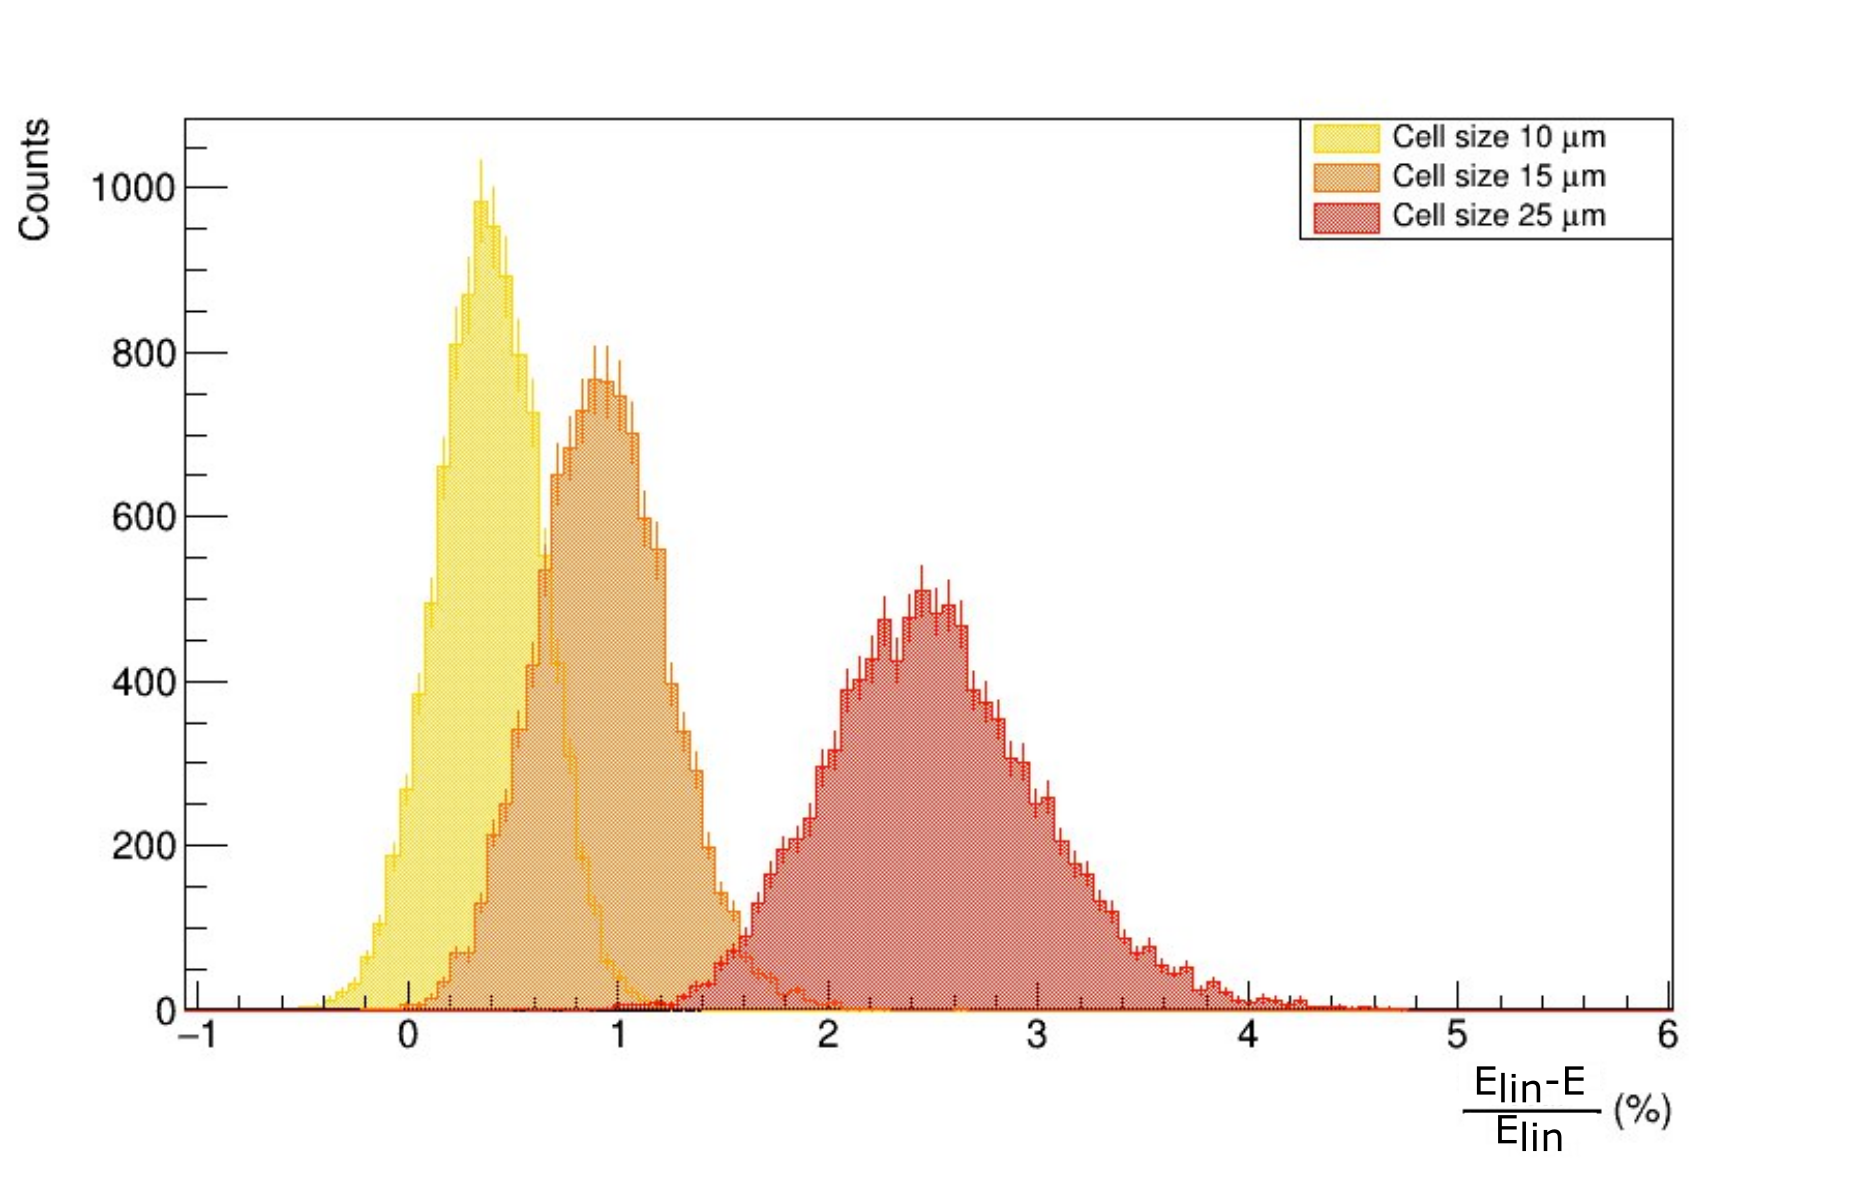
\includegraphics[width=.85\textwidth]{IMG/Cap5/PercEnergy_40GeV_cher.png}} \quad
	\subfloat[][Scintillation signals.]{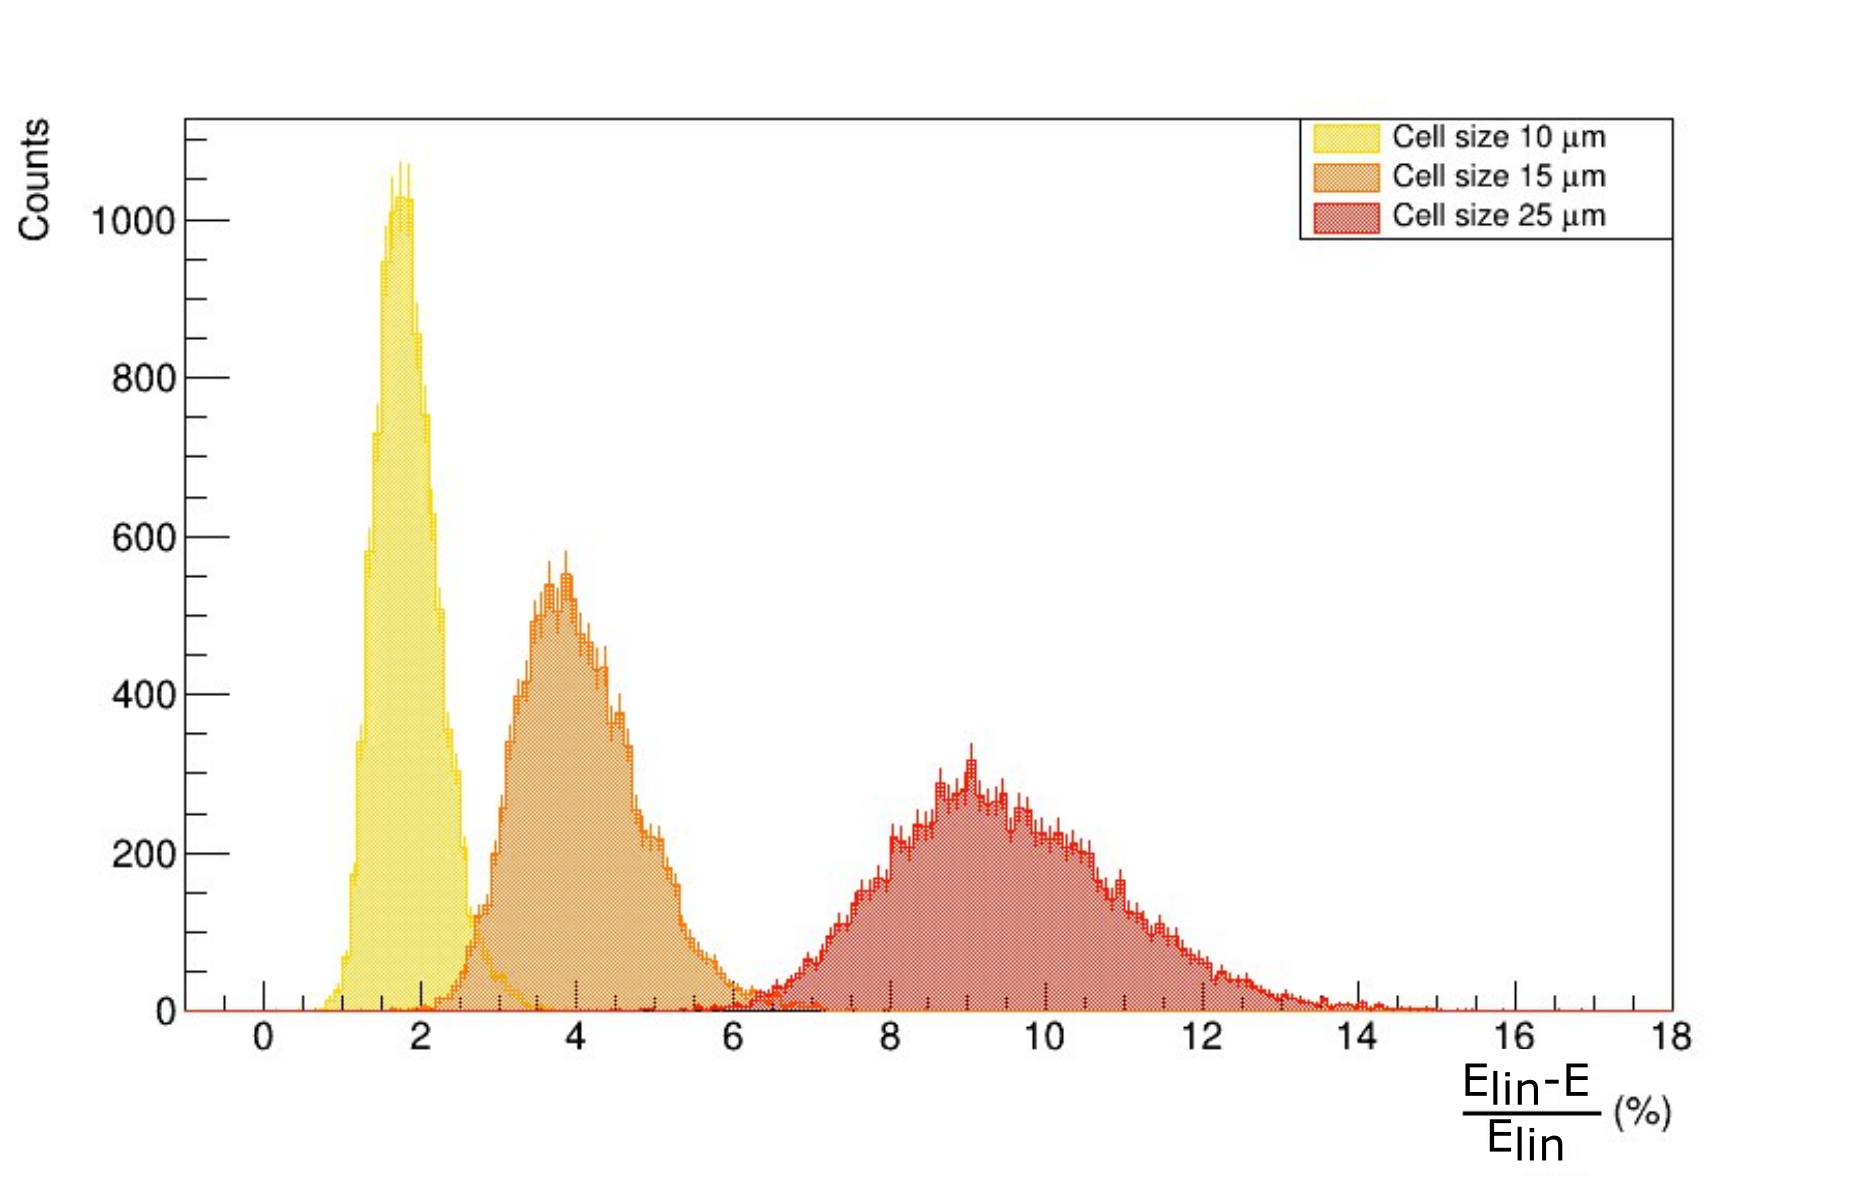
\includegraphics[width=.85\textwidth]{IMG/Cap5/PercEnergy_40GeV_scin.png}}
	\caption{Percentage discrepancy distribution considering events with single 40~GeV electrons. Different colours correspond to different cell-size values.}
	\label{fig:perc_sat}
\end{figure}

\begin{figure}
	\centering
	\subfloat[][Cherenkov signals.]{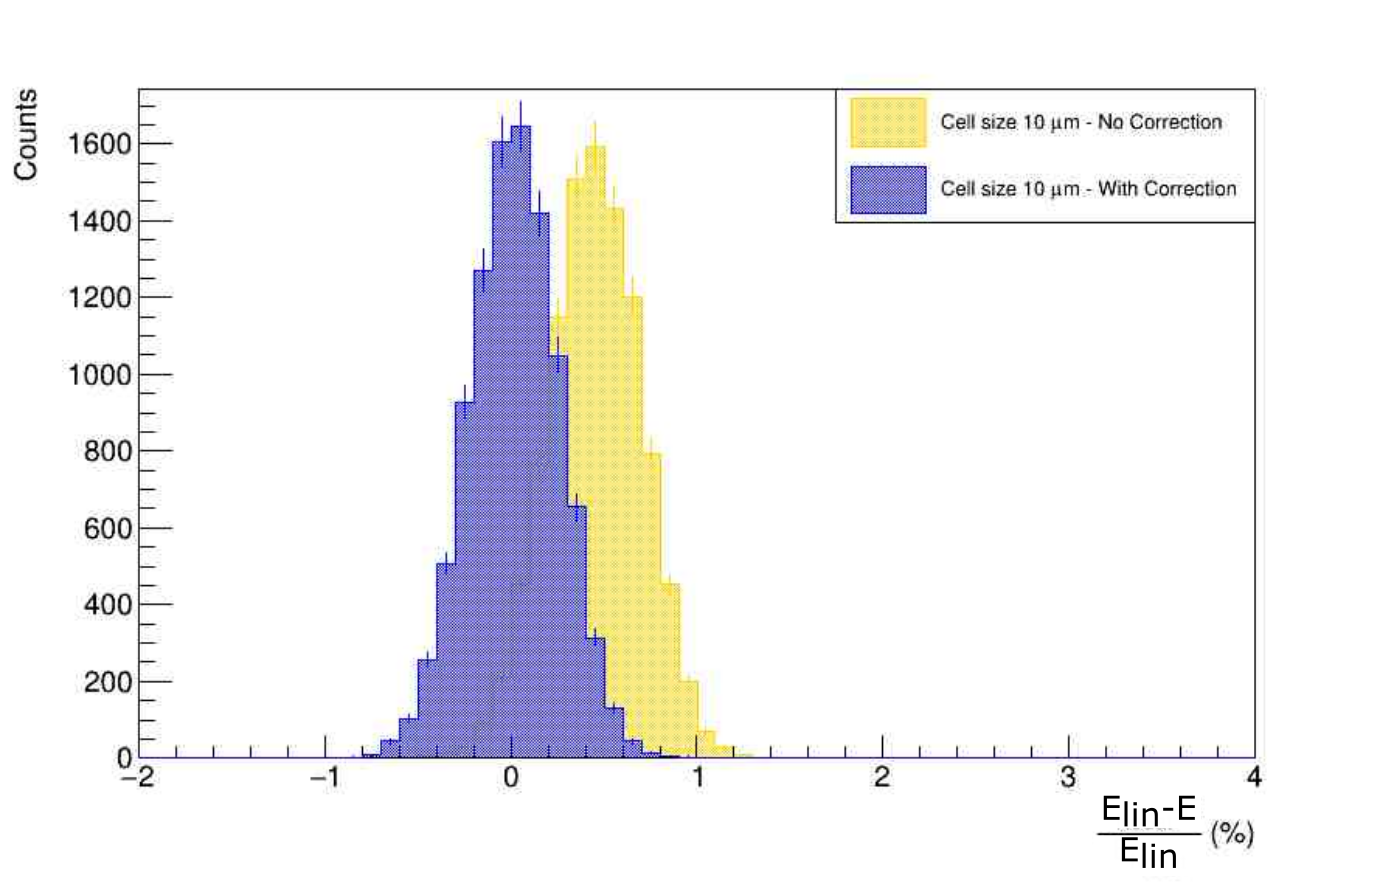
\includegraphics[width=.85\textwidth]{IMG/Cap5/PercEnergy_40GeV_corr_cher.png}} \quad
	\subfloat[][Scintillation signals.]{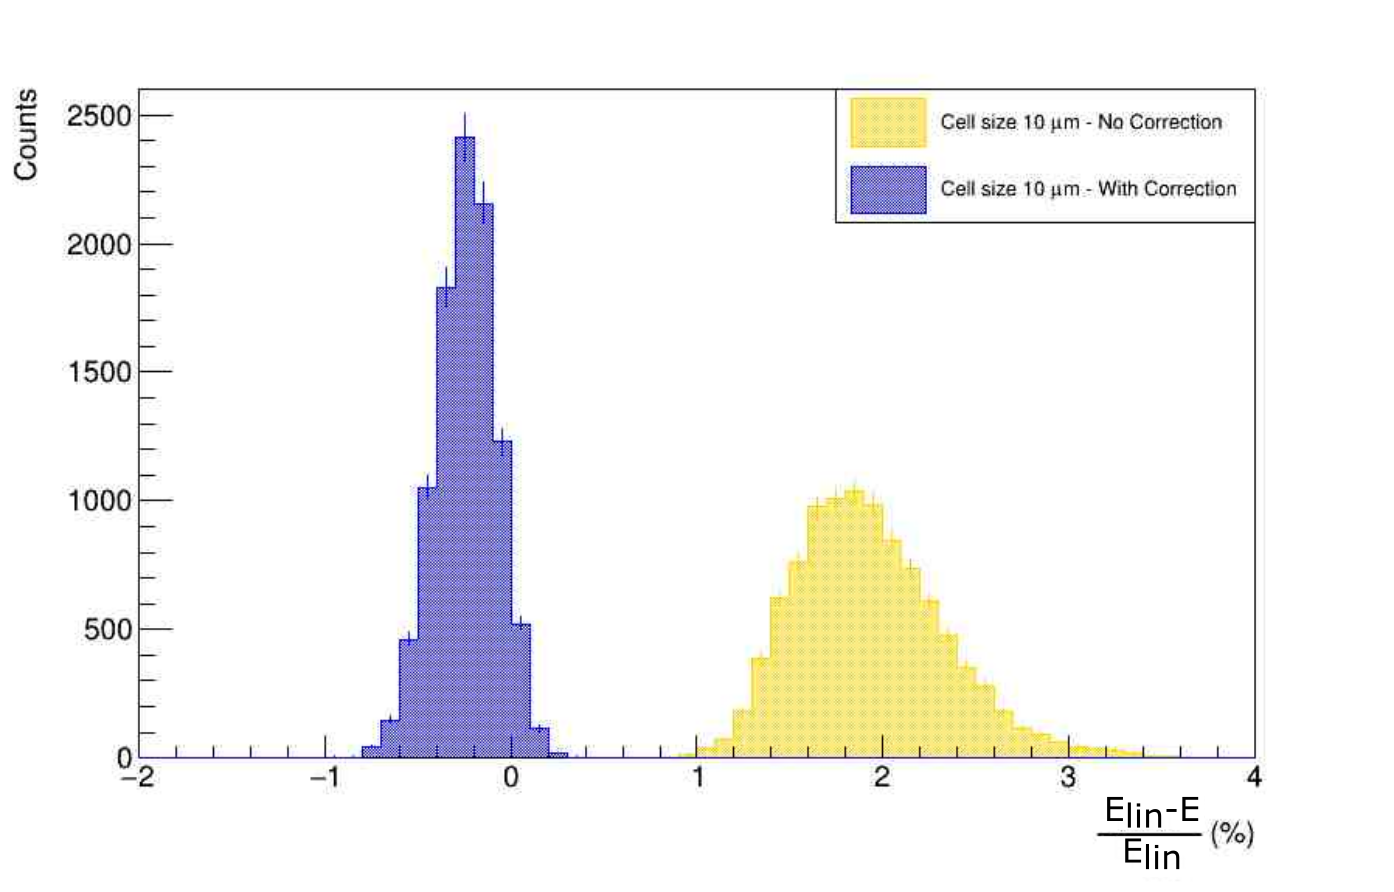
\includegraphics[width=.85\textwidth]{IMG/Cap5/PercEnergy_40GeV_corr_scin.png}}
	\caption{Percentage discrepancy distribution considering events with single 40~GeV electrons to evaluate the effect of the analytical correction applied on data obtained with a cell size of $10$ $\mu$m.}
		\label{fig:sat_corr_perc}
\end{figure}

This whole process has been performed simulating electrons with energies of $20,\ 40,\ 60$ and $80$ GeV. Mean and standard deviation of the gaussian fit of the percentage discrepancy have been recorded and their values are plotted in Figure \ref{fig:sat_vs_E} where a non-linearity well below the $1\%$ is obtained for both Cherenkov and scintillation signals, after applying the analytical corrections for a $10~\mu$m cell size.\\

\begin{figure}
	\centering
	\subfloat[][Cherenkov signals.]{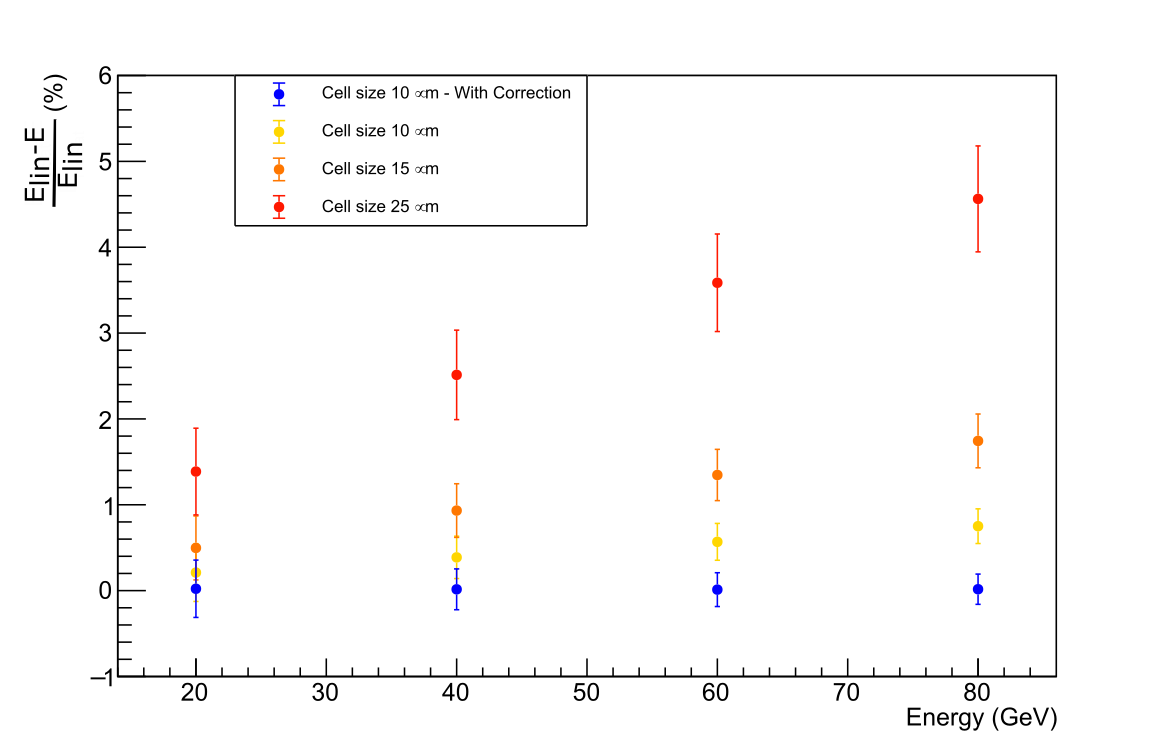
\includegraphics[width=.85\textwidth]{IMG/Cap5/PercEnergy_cher.png}} \\
	\subfloat[][Scintillation signals.]{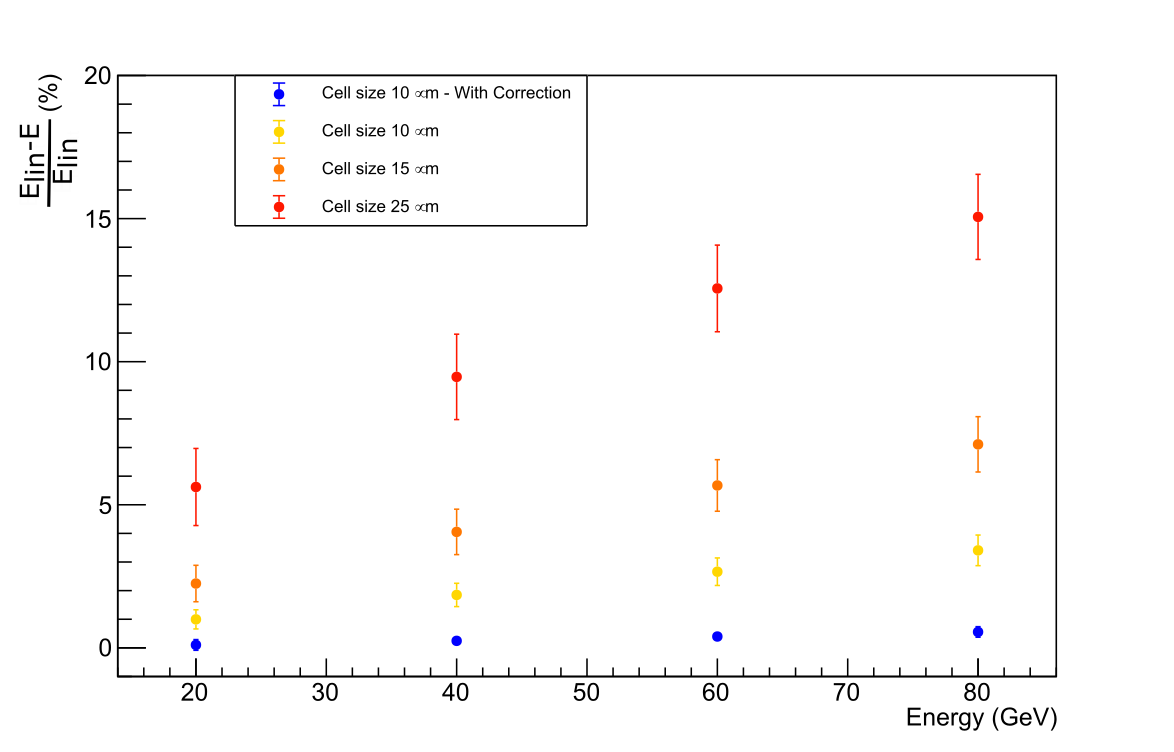
\includegraphics[width=.85\textwidth]{IMG/Cap5/PercEnergy_scin.png}}
	\caption{Percentage discrepancy behaviour with respect to the primary particle energy. The results for the different cell sizes are shown, also compared with the results obtained performing the analytical correction to the $10~\mu$m cell-size data.}
	\label{fig:sat_vs_E}
\end{figure}

\subsection{Energy resolution} \label{subsec:E_res}
Dual-readout calorimeters are typically calibrated at the electromagnetic scale. This is especially useful in a leptonic collider because, having easily access to reference "candles" such as  electrons and positrons from Z decays, the calorimeter can be precisely calibrated during all the life of the experiment.\\
The first step to study the energy resolution is to calibrate the calorimeter.\\

The calibration has been performed with $40$ GeV electrons applying the 1.5pe-suppression already introduced in Paragraph \ref{subsec:Sim_SiPM}. $10000$ events with single $40$ GeV electrons have been fired from the interaction point obtaining the charge integral distributions for scintillation and Cherenkov signals.% shown in Figure \ref{fig:int_dist}.
The calibration constants obtained to transform these data in energy distributions centred around $40$ GeV are: $k_S = 4.998 \times 10^{-5}$ GeV$/$A.U. and $k_C = 2.023 \times 10^{-4}$ GeV$/$A.U.\\
Two analogue calibration constants have been obtained starting from the number of photoelectron distribution with values of: $k_{pe,S} = 2.48 \times 10^{-3}$ GeV$/$p.e. and $k_{pe,C} = 1.00 \times 10^{-2}$ GeV$/$p.e..\\

%\begin{figure}
%	\centering
%	\subfloat[][Cherenkov signals.]{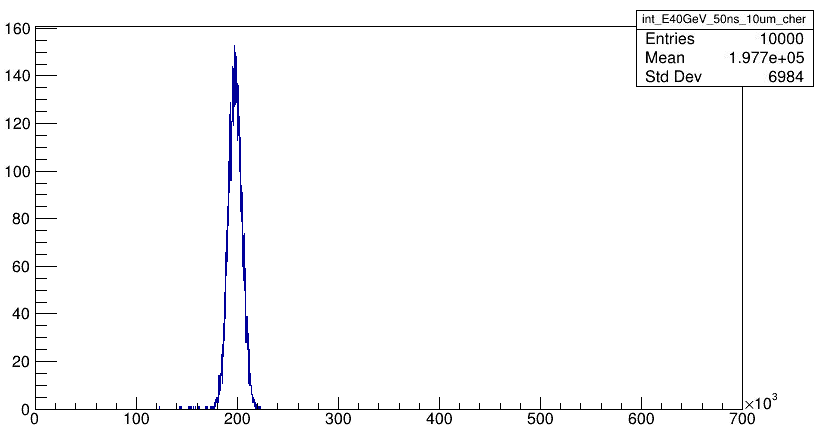
\includegraphics[width=.7\textwidth]{IMG/Intdist_40GeV_cher_cal}} \\
%	\subfloat[][Scintillation signals.]{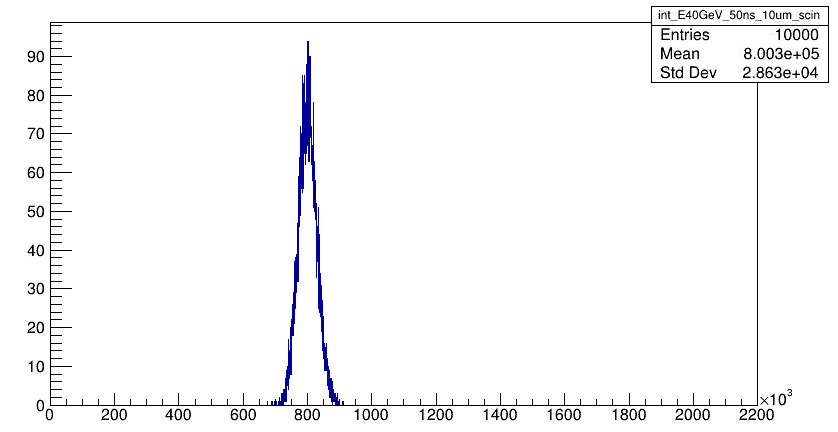
\includegraphics[width=.7\textwidth]{IMG/Intdist_40GeV_scin_cal}}
%	\caption{Integral distrib.}
%	\label{fig:int_dist}
%\end{figure}

Starting from these calibration constants, the energy distributions can be obtained either from the number of p.e.s (pre SiPM digitisation simulation) or from the charge integral (post SiPM digitisation simulation). The two types of distribution are compared in Figure \ref{fig:cfr_e_dist}.\\
The energy distributions obtained from the charge integrals are slightly wider, as expected due to the introduction of the electronic noise. However, the effect is really minimal considering the fact that, in each event, hundreds of SiPMs are active.\\
%and the white noise has mean zero.

\begin{figure}
	\centering
	\subfloat[][Cherenkov signals.]{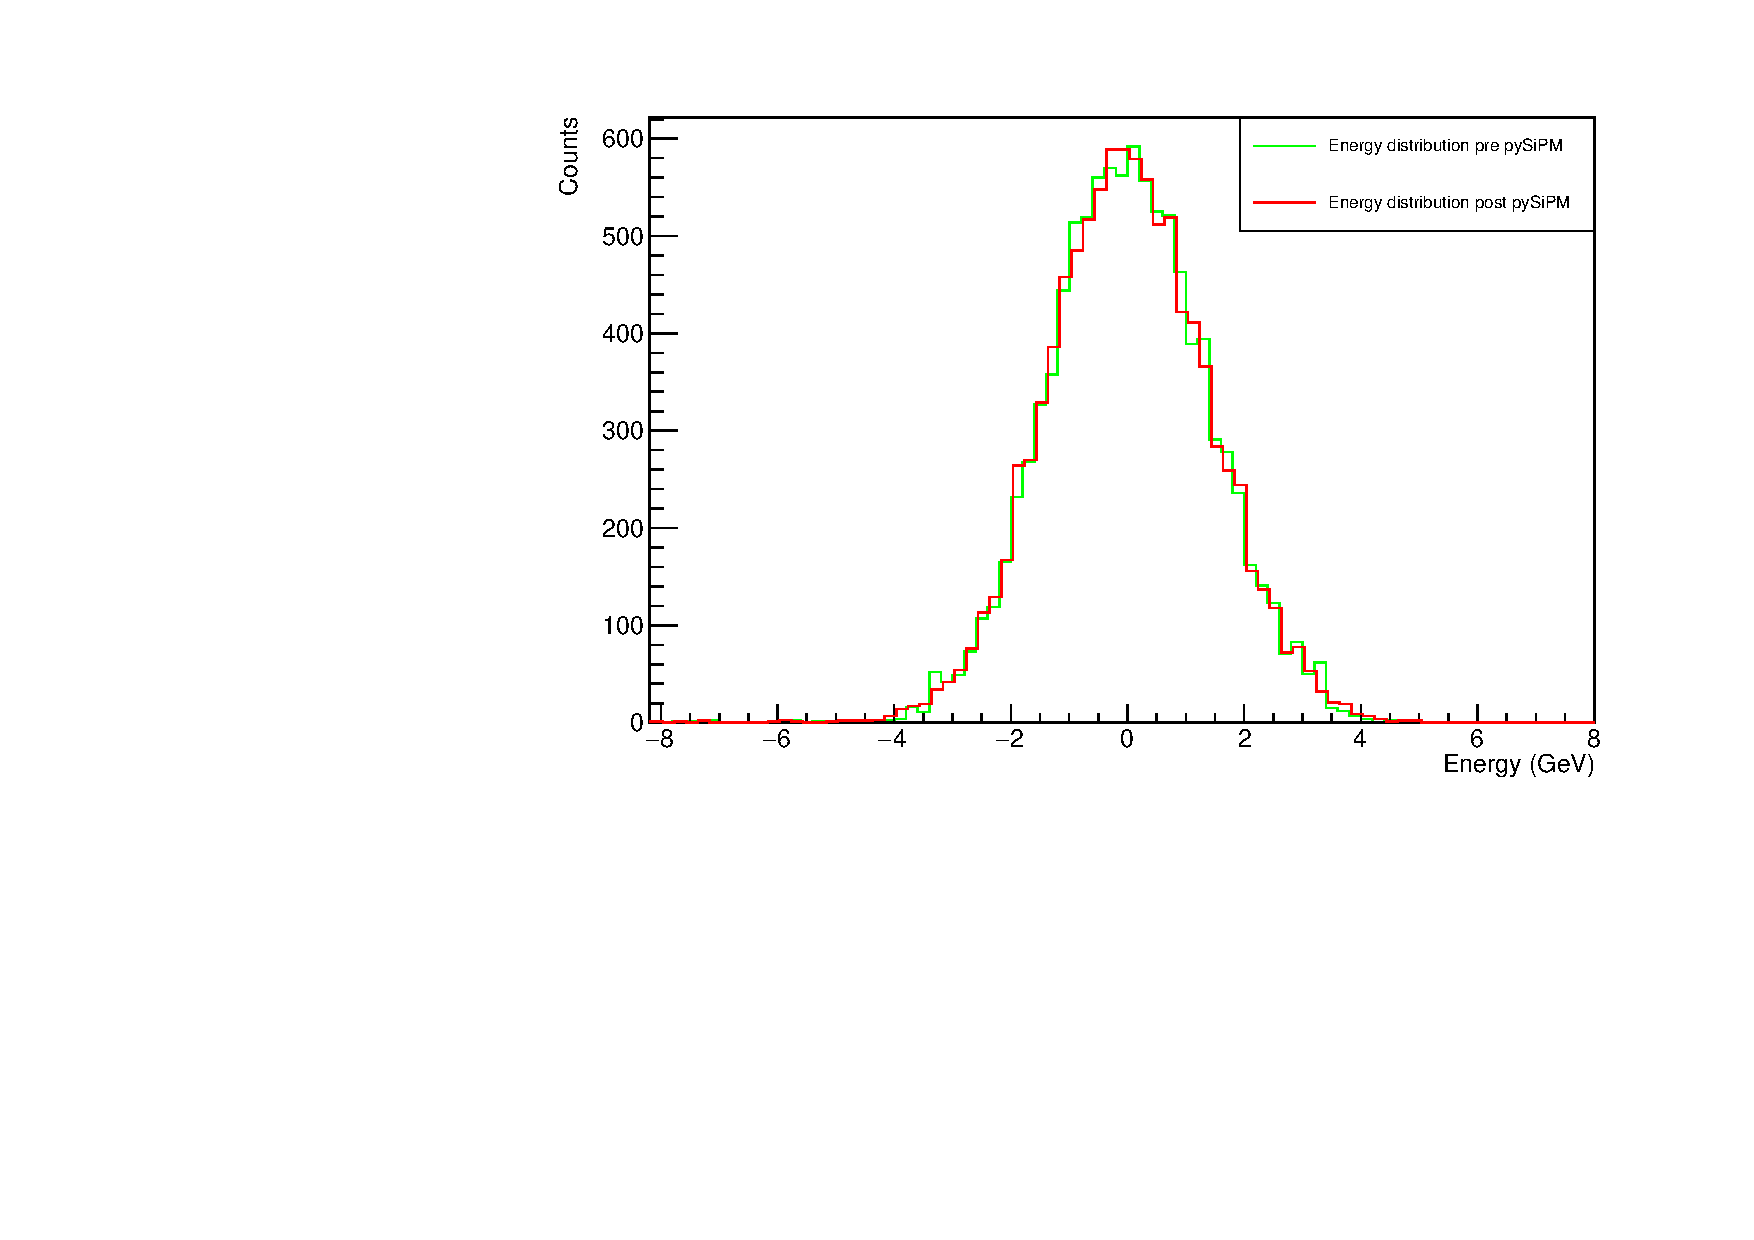
\includegraphics[width=.85\textwidth]{IMG/Cap5/E_hist_cfr_cher}} \\
	\subfloat[][Scintillation signals.]{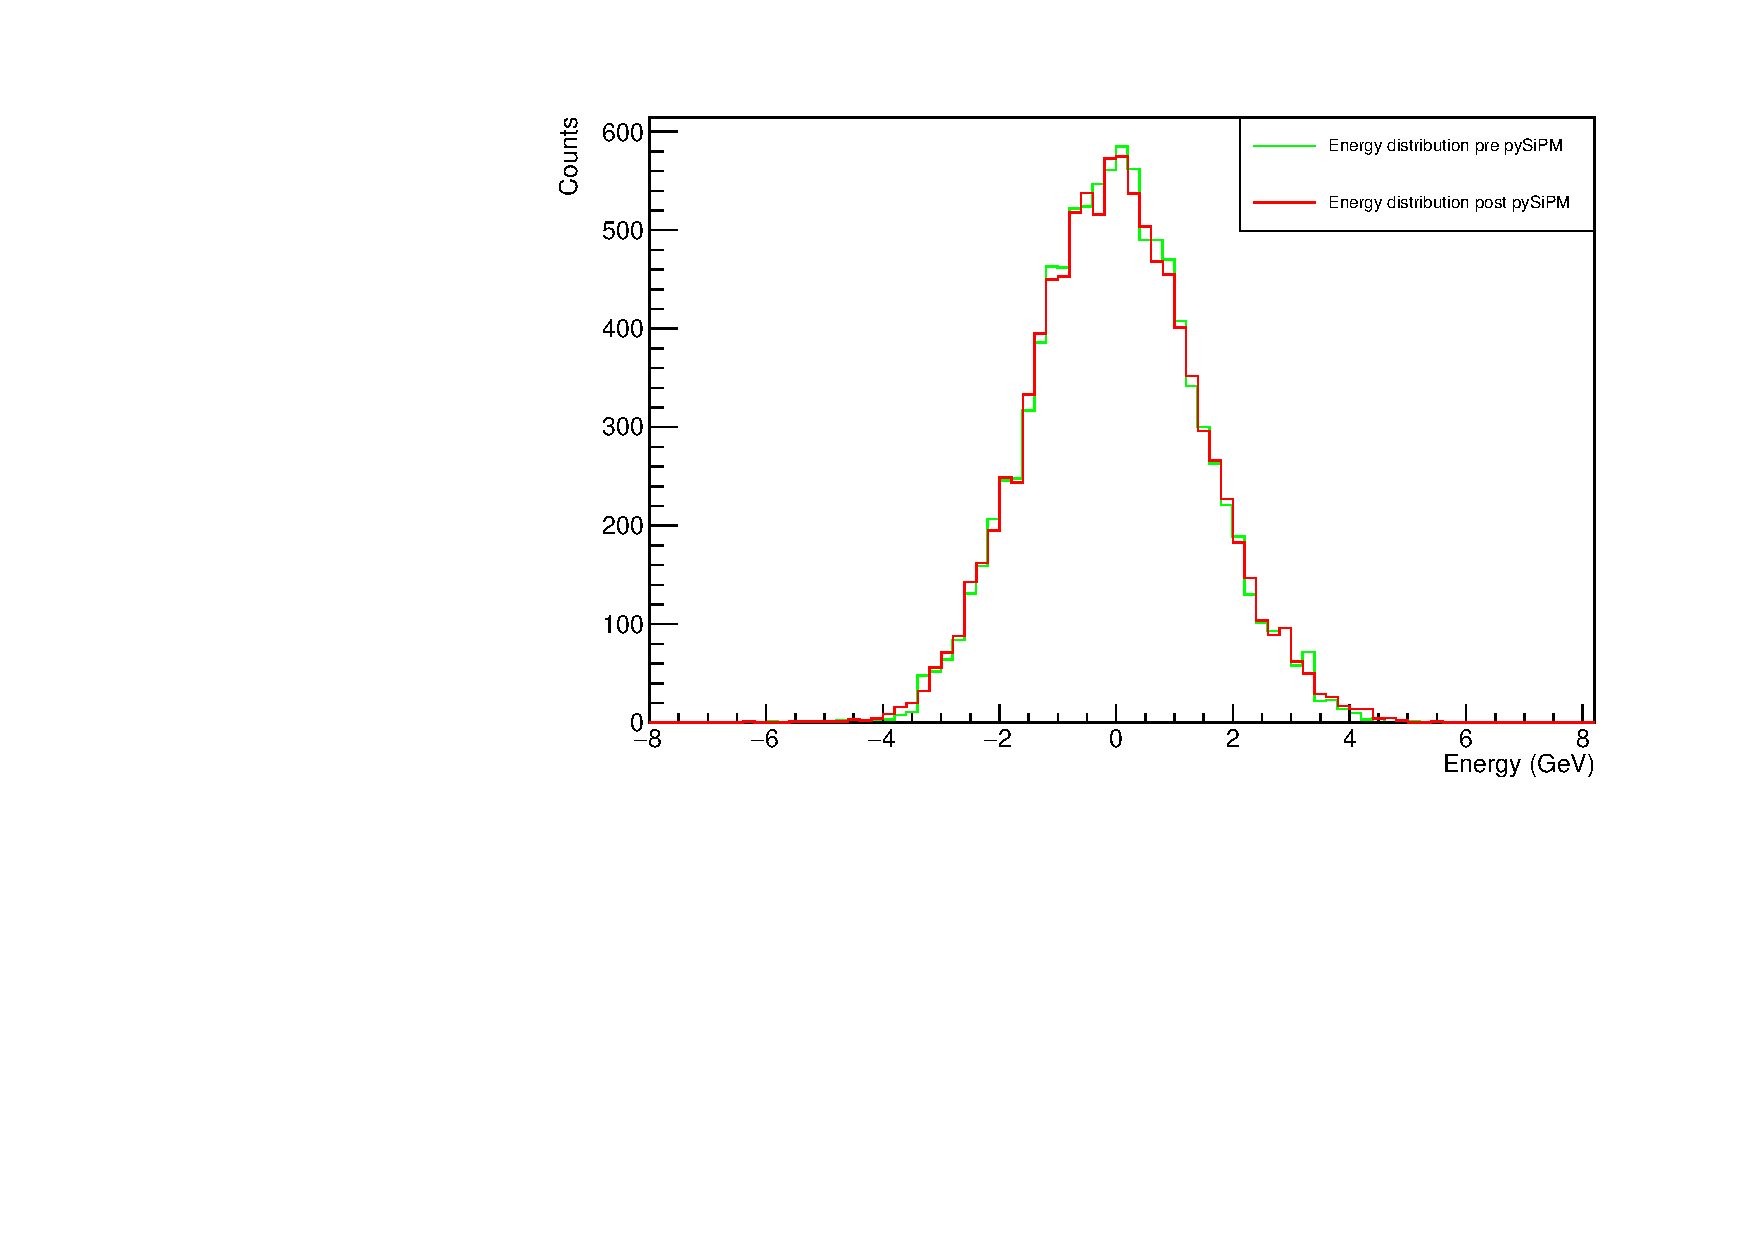
\includegraphics[width=.85\textwidth]{IMG/Cap5/E_hist_cfr_scin}}
	\caption{Charge integral distributions generated with data from GEANT4 (\textit{pre pySiPM}) or from the full simulation (\textit{post pySiPM}). The mean values (that, however, have very little differences) have been subtracted.}
	\label{fig:cfr_e_dist}
\end{figure}

The energy distributions have been fitted with a Gaussian function to obtain mean, standard deviation and the respective errors. By doing this with different primary electron energies, the energy resolution can be studied. Mean and standard deviation are listed in Table \ref{tab:e_res_pe}.\\
Then, fitting the $\sigma/E$ values obtained from photoelectron number in the energy range $5-80$ GeV, it can be seen that the distribution is well described by the function:
\begin{equation}\label{eq:resolution}
	\frac{\sigma}{E} = \frac{A}{\sqrt{E}} \oplus B,
\end{equation} 
with parameter values of $A = 18.97\%$ and $B = 1.677\%$, for scintillation signals, and $A = 21.01\%$ and $B = 0.386\%$, for Cherenkov signals.\\
On the other hand, adding the SiPM digitization, an uncorrelated electronics noise contribution scaling as $C/E$ has to be added in quadrature.\\
The plots in Figure \ref{fig:sigma_su_e} show that the energy resolution points after the SiPM digitization are almost identical with respect to the one obtained from the calorimeter-only simulation data. Therefore the impact on the resolution, due the introduction of the SiPM simulation software, is negligible.
%, therefore the fit function became:
%\begin{equation}\label{eq:resolution2}
%	%\frac{\sigma}{E} = \frac{A_1}{\sqrt{E}} + B_1 \qquad \text{or} \qquad \frac{\sigma}{E} = \frac{A_2}{\sqrt{E}} \oplus B_2
%	\frac{\sigma}{E} = \frac{A}{\sqrt{E}} \oplus B \oplus \frac{C}{E},
%\end{equation} 
%where the parameters $A$ and $B$, that in first approximation should not be affected by the digitization, have been fixed as the one obtained before. The plots are shown in Figure \ref{fig:sigma_su_e}, with the fit parameters listed in Table \ref{tab:res_regular_sum}. They also show that the loss of resolution with the introduction of the SiPM digitization software is minimal.\\
% and \ref{tab:res_quadratic_sum}

\begin{table}
	\centering
	\begin{tabular}{lccc}
	    \toprule
	    \multicolumn{4}{c}{\textbf{Pre pySiPM}}\\
		\midrule
		& True E (GeV) & Mean E (GeV) & Standard Deviation (GeV) \\
		\midrule
		\textbf{Scintillation} &	$5$ 	& $4.91$ & $0.41$ \\
		& $20$ 	& $19.90$ & $0.92$ \\
		& $40$ 	& $40.00$ & $1.39$ \\
		& $60$ 	& $60.65$ & $1.78$ \\
		& $80$ 	& $81.18$ & $2.16$ \\
		\midrule
		\textbf{Cherenkov} & $5$ 	& $4.77$ & $0.48$ \\
		& $20$ 	& $19.76$ & $0.92$ \\
		& $40$ 	& $40.00$ & $1.36$ \\
		& $60$ 	& $60.40$ & $1.66$ \\
		& $80$ 	& $81.86$ & $1.91$ \\
		\toprule
	    \multicolumn{4}{c}{\textbf{Post pySiPM}}\\
		\midrule
		& True E (GeV) & Mean E (GeV) & Standard Deviation (GeV) \\
		\midrule
		\textbf{Scintillation} &	$5$ 	& $4.91$ & $0.42$ \\
		& $20$ 	& $19.90$ & $0.92$ \\
		& $40$ 	& $40.00$ & $1.42$ \\
		& $60$ 	& $60.65$ & $1.83$ \\
		& $80$ 	& $81.18$ & $2.22$ \\
		\midrule
		\textbf{Cherenkov} & $5$ 	& $4.80$ & $0.45$ \\
		& $20$ 	& $19.88$ & $0.91$ \\
		& $40$ 	& $40.00$ & $1.36$ \\
		& $60$ 	& $60.63$ & $1.66$ \\
		& $80$ 	& $81.12$ & $1.92$ \\
		\bottomrule
	\end{tabular}
	\caption{Mean and standard deviation obtained by fitting with Gaussian function the energy distributions. The data are obtained with results from DR calorimeter simulation applying the calibration from the photoelectron number in the top rows and with results from the full simulation in the bottom rows.}
	\label{tab:e_res_pe}
\end{table}

\begin{figure}
	\centering
	\subfloat[][$C$ signals.]{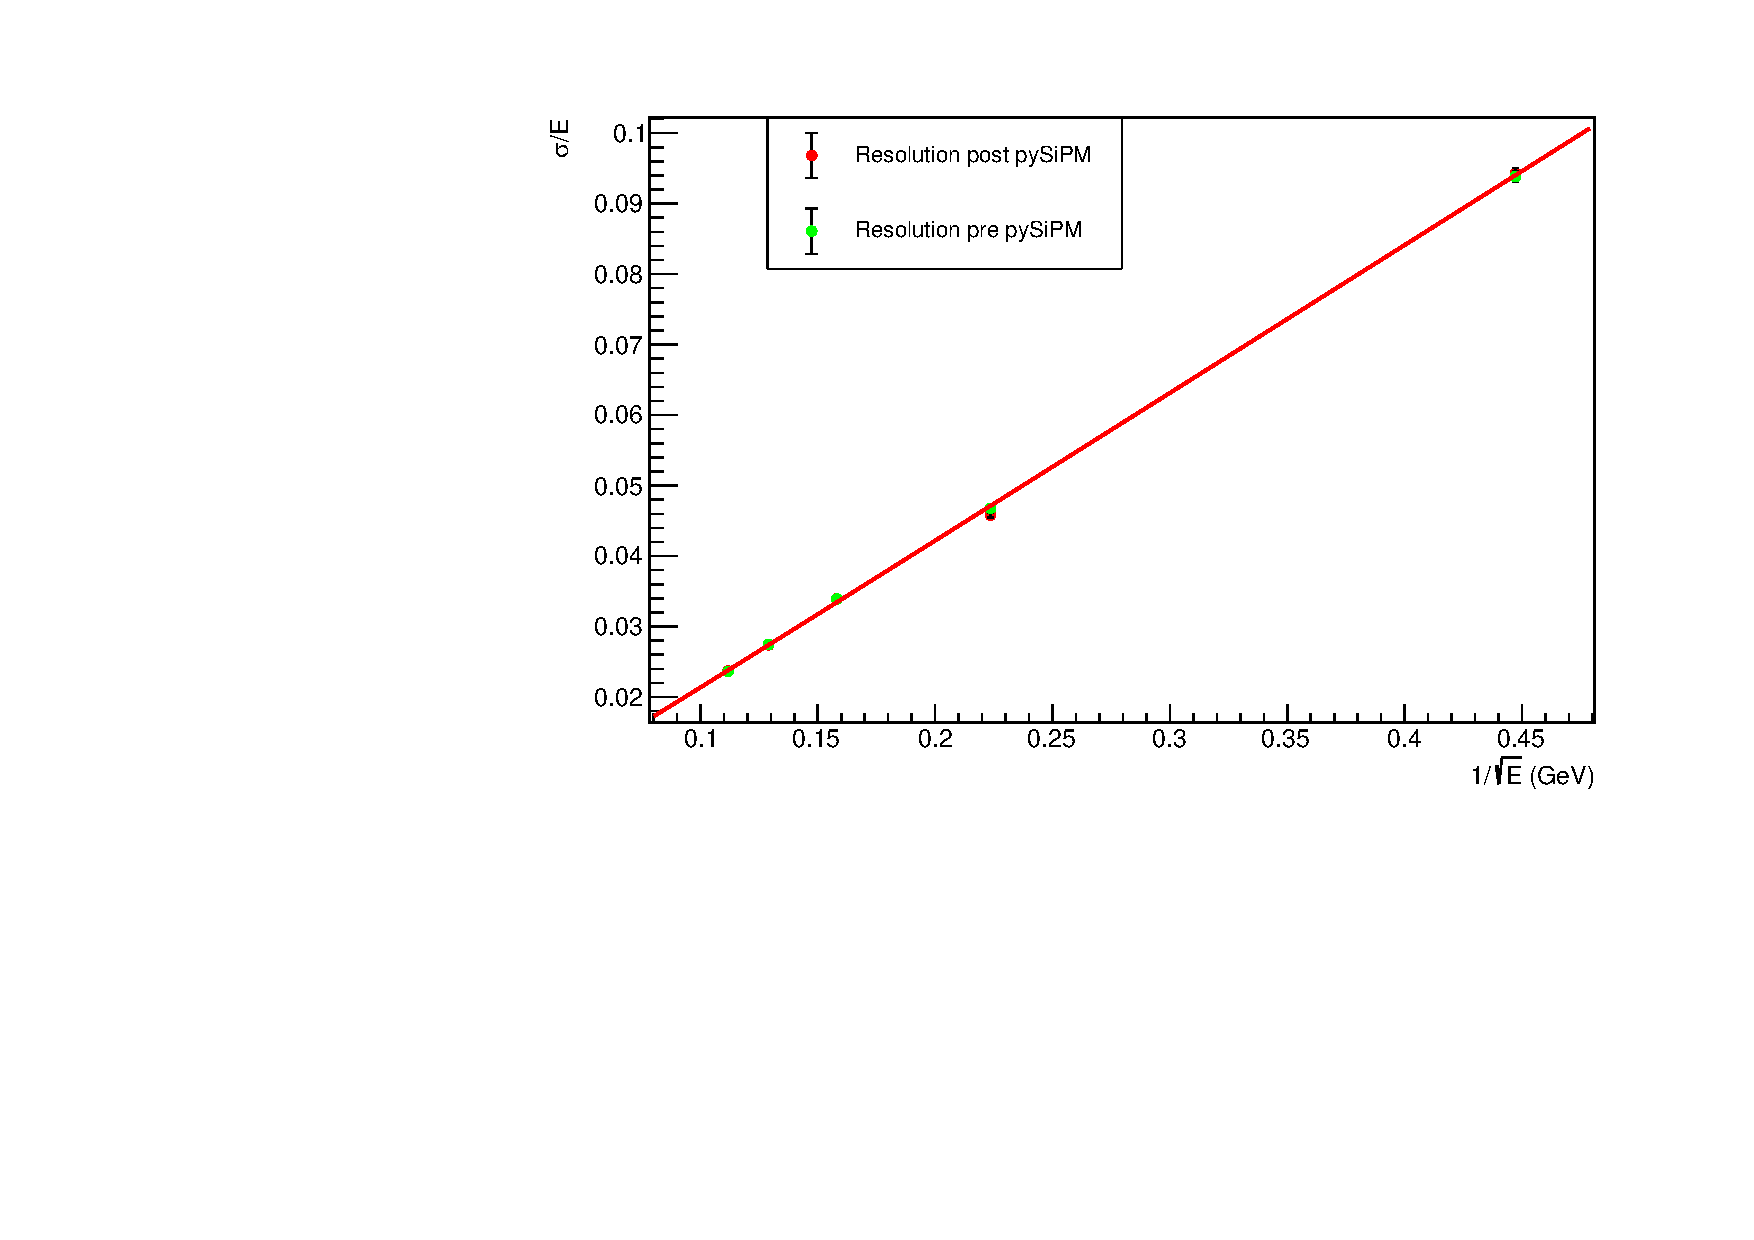
\includegraphics[width=.85\textwidth]{IMG/Cap5/Res_cher.pdf}} \\
	\subfloat[][$S$ signals.]{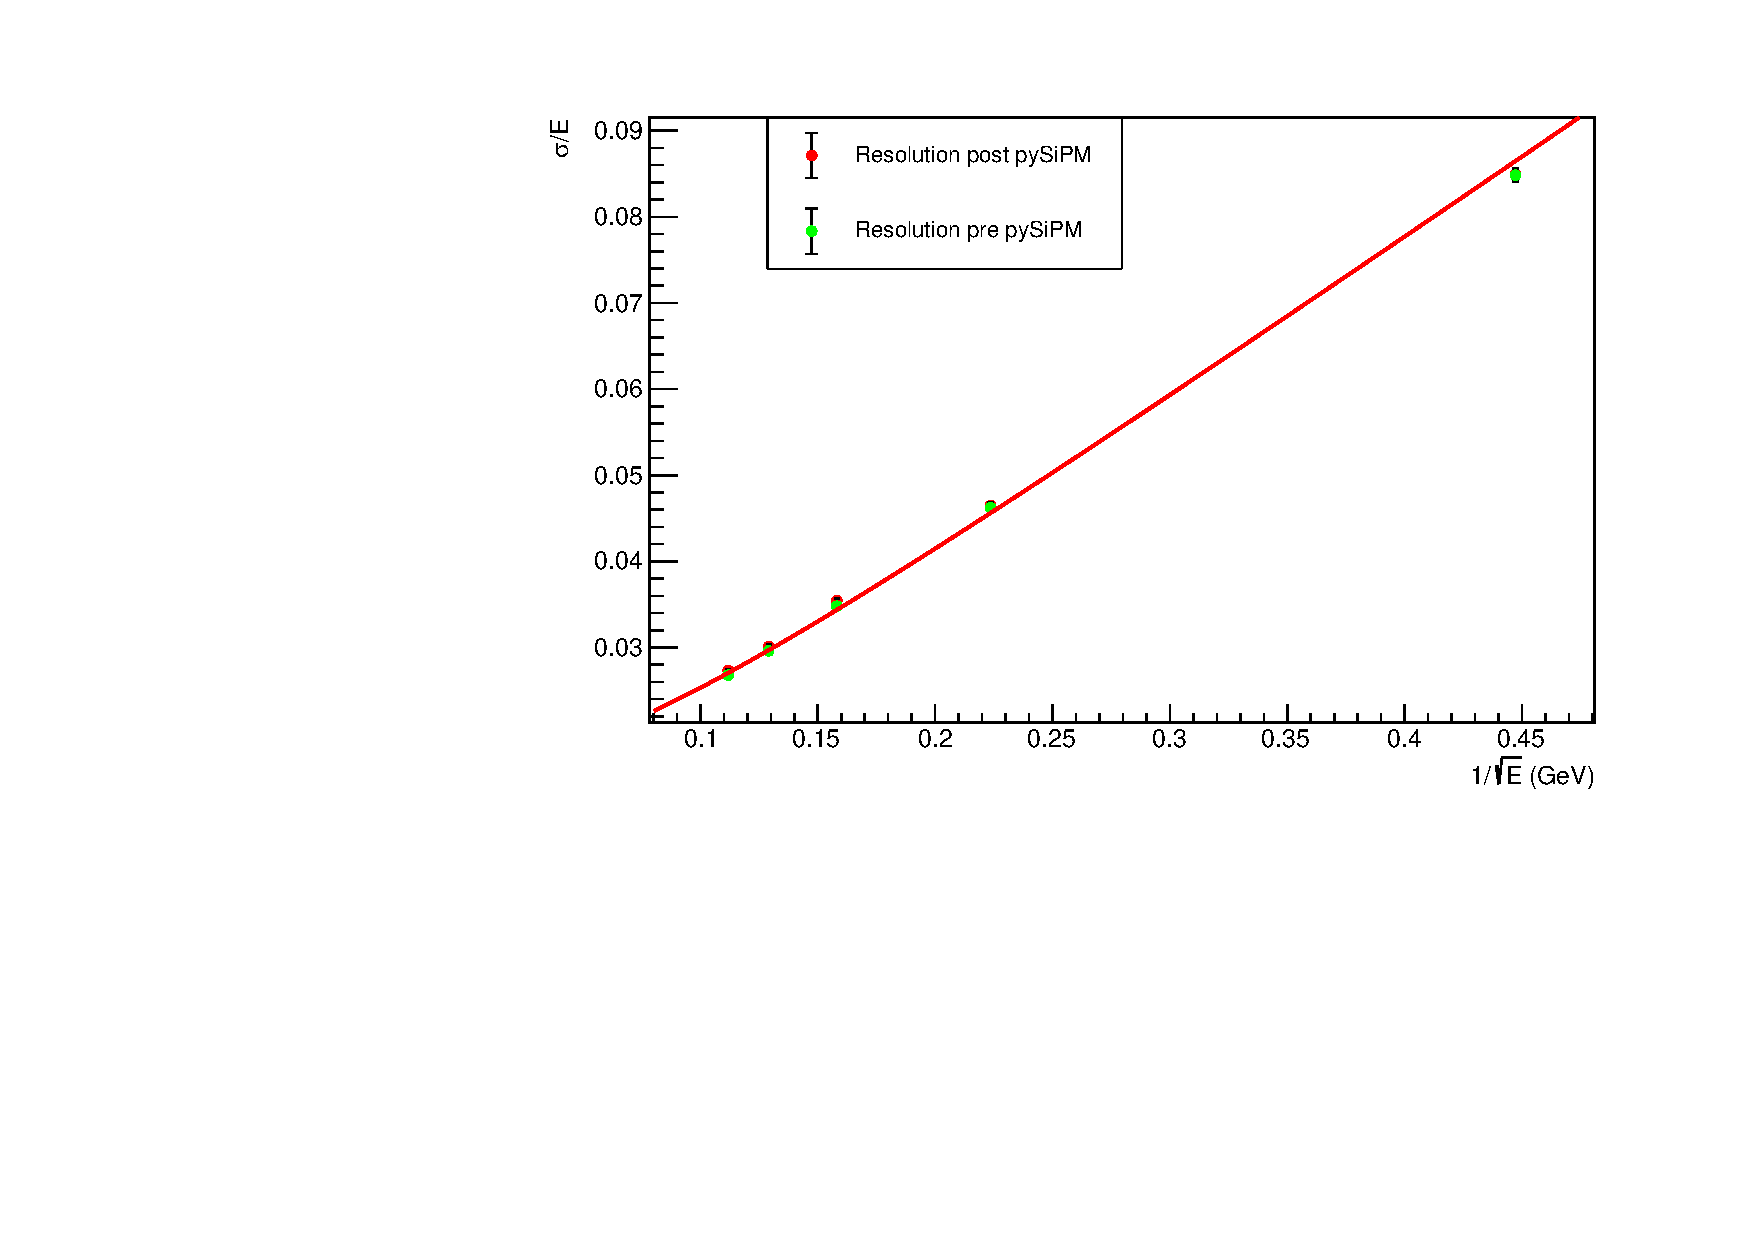
\includegraphics[width=.85\textwidth]{IMG/Cap5/Res_scin.pdf}}
	\caption{Calorimeter resolution plot where the data have been fitted with the Formula \ref{eq:resolution}.}
	\label{fig:sigma_su_e}
\end{figure}